\clearpage

\section {Validation of the \textit{VALOR} Run1+2+3+4 joint 3-flavour oscillation analysis: study of fitter performance at 6.5700 $\times$10$^{20}$ POT}
\label{sec:validation}

Different studies were made in order to validate the \textit{VALOR} Run1+2+3+4 joint 3-flavour oscillation analysis. In this section, a summary of the studies concerning the fitter performance are presented. The implementation of each systematic and its effect in the proper modes and templates has been carefully studied and reported in an additional document that can be found together with this technical note \cite{AdditionalMaterial}.

\subsection{Residuals and pulls for the oscillation parameters}

The residuals and pulls presented in this section were obtained using 5k toy MC experiments generated with statistical fluctuations and variations of all 64 systematic parameters, fitting them using MINUIT and computing the MINUIT HESSE errors. In order to avoid effects of physical boundaries, the following study was made at the oscillation point $sin^{2}\theta_{23} = 0.5263$ and $sin^{2}\theta_{13} = 0.05$. The value for $sin^{2}\theta_{13}$ was selected to be large enough to avoid the effect of the physical boundary at $sin^{2}\theta_{13} = 0$ that could be observed as an asymmetry in the distribution of residuals if a small value of $sin^{2}\theta_{13}$ is used. For the other angle $sin^{2}\theta_{23}$ the value was selected to be in the point of maximal disappearance given that $sin^{2}\theta_{13} = 0.05$, which is calculated as $\approx (2(1-sin^{2}\theta_{13}))^{-1}$ according to the explanation in Appendix E of \cite{OurJointAnalysis}. The other oscillation parameters were set to $\Delta m^{2} = 2.4 \times 10^{-3} eV^{2}/c^{4}$ and $\delta_{CP} = 0$, and normal hierarchy was assumed. 

Figures \ref{fig:validation:residuals} and \ref{fig:validation:pulls} show the distribution of residuals and pulls respectively of the four oscillation parameters at the oscillation point $sin^{2}\theta_{23} = 0.5263$, $sin^{2}\theta_{13} = 0.05$, $\Delta m^{2} = 2.4 \times 10^{-3} eV^{2}/c^{4}$ and $\delta_{CP} = 0$ and normal hierarchy for an ensemble of 5k toy MC experiments. Residuals and pulls of only the events which are at the central peak in $sin^{2}\theta_{23}$ are presented in Figs. \ref{fig:validation:residuals_central} and \ref{fig:validation:pulls_central}. For the other two peaks away from the true value of $sin^{2}\theta_{23}$ residuals and pulls are shown in Figs. \ref{fig:validation:residuals_peaks} and \ref{fig:validation:pulls_peaks}. Since one of the two peaks is reduced in the joint fit, these figures show the distributions from the two independent fist performed with an initial value in each octant, before selecting the one with minimal $\chi^{2}$. 

Fig \ref{fig:validation:residuals_fixdcp} shows the distribution of residuals and pulls respectively of the four oscillation parameters at the oscillation point $sin^{2}\theta_{23} = 0.5263$, $sin^{2}\theta_{13} = 0.05$, $\Delta m^{2} = 2.4 \times 10^{-3} eV^{2}/c^{4}$ and $\delta_{CP} = 0$ and normal hierarchy for an ensemble of 4k toy MC experiments fixing $\delta_{CP} $ to its true value, and Fig. \ref{fig:validation:residuals_central_fixdcp} selecting only the events which are at the central peak in $sin^{2}\theta_{23}$.

From the study of residuals and pulls the following features can be observed:

\begin{itemize}
\item{\textbf{Three peak structure in $sin^{2}\theta_{23}$}

The three peak structure in the residuals for $sin^{2}\theta_{23}$ observed in Fig. \ref{fig:validation:residuals}
and the specific location of the two extra peaks away from the true value 
is a known feature of this parameter which has been explained in detail in the validation of the
\textit{VALOR} Run1+2+3+4 $\nu_{\mu}$ disappearance analysis in \cite{OurRun1234DisappAnalysis3Flavour}.
One of the two peaks away from the true value (the one corresponding to the solution in the second octant) is 
suppressed when the contribution to the total $\chi^{2}$ coming from the single e-like ring sample is added
(it was checked that when using only the $\chi^{2}$ contribution from the single $\mu$-like ring sample 
both peaks appeared). The explanation for this suppression will be given in a later bullet.

Comparing Fig. \ref{fig:validation:residuals_central} with Fig. \ref{fig:validation:residuals_peaks} and
Fig. \ref{fig:validation:pulls_central} with Fig. \ref{fig:validation:pulls_peaks} it is clear that the main
source for the biases in the distribution of residuals for $\Delta m^{2}$ and $sin^{2}\theta_{13}$
comes from the extra peaks away from the true value. 
}


\item{\textbf{Intrinsic asymmetry in $sin^{2}\theta_{13}$-$\delta_{CP}$}

It was observed that an intrinsic asymmetry exist in the $sin^{2}\theta_{13}$-$\delta_{CP}$ space. 
This asymmetry is clear when looking at the true $\Delta\chi^{2}$ distribution for the single e-like ring sample
in the ($sin^{2}\theta_{13}$,$\delta_{CP}$) space for a toy created at the oscillation point 
$sin^{2}\theta_{23} = 0.5263$, $sin^{2}\theta_{13} = 0.05$, $\Delta m^{2} = 2.4 \times 10^{-3} eV^{2}/c^{4}$ and $\delta_{CP} = 0$
assuming normal hierarchy without statistical fluctuations nor systematic variations in Fig. \ref{fig:validation:truechisq}. 
In this figure, the region of minimal $\Delta\chi^{2}$ is clearly not centered at  $\delta_{CP} = 0$, $sin^{2}\theta_{13} = 0.05$ (the true value)
but it is asymmetric, centered at a value $\delta_{CP}>0$ and $sin^{2}\theta_{13}>0.05$. 
This explains the fact that when creating toy experiments with statistical and systematic variations, the center of the distribution of
residuals for $\delta_{CP}$ is not center at 0 but at $\delta_{CP}\approx 0.6$ even when removing other sources that could create a bias (fixing $sin^{2}\theta_{23}$ to
its true value for instance) as observed for example in Fig. \ref{fig:validation:residuals}.
This asymmetry and consequent bias in $\delta_{CP}$ causes also a bias to values $sin^{2}\theta_{13}>0.05$.


This is a direct consequence of the energy spectrum of T2K event candidates convoluted with the oscillation probability
$P(\nu_{\mu}\rightarrow\nu_{e})$. Figure \ref{fig:validation:biasdeltacp} (left) shows the true energy spectrum for the single e-like ring
event candidates for the oscillated $\nu_{e}$ category in the T2K SKMC, zooming around the peak of the spectrum. On the right part 
of Fig. \ref{fig:validation:biasdeltacp} lines of equal $\Delta(P(\nu_{\mu}\rightarrow\nu_{e}))$ are drawn for the different values of the true energy
at the peak of the spectrum on the left side (from 0.45 GeV to 0.85 GeV). The $\Delta(P(\nu_{\mu}\rightarrow\nu_{e}))$ to draw these 
lines is selected with respect to the oscillation probability at the true values 
$sin^{2}\theta_{23} = 0.5263$, $sin^{2}\theta_{13} = 0.05$, $\Delta m^{2} = 2.4 \times 10^{-3} eV^{2}/c^{4}$ and $\delta_{CP} = 0$
(in a range of $\Delta(P(\nu_{\mu}\rightarrow\nu_{e})) < 0.005$) for each different true energy. Red regions indicates points where all the oscillation probability 
lines crossed, so points where approximately the same oscillation probability is obtained for the different true energies of the peak 
on the right. That translates into points where the $\Delta\chi^{2}$ value will be approximately the same, minimal with respect to 
the true oscillation point. The shape and position of the red region in the left side of Fig. \ref{fig:validation:biasdeltacp}
describes exactly the asymmetry observed in Fig. \ref{fig:validation:truechisq}. 

The true values of other oscillation parameters except $\delta_{CP}$ do not affect the position of this region 
as can be observed in Fig. \ref{fig:validation:biasdeltacp2}, where the oscillation point is 
 $sin^{2}\theta_{23} = 0.5263$, $sin^{2}\theta_{13} = 0.03$, $\Delta m^{2} = 2.4 \times 10^{-3} eV^{2}/c^{4}$ and $\delta_{CP} = 0$ on the left plot
and $sin^{2}\theta_{23} = 0.3$, $sin^{2}\theta_{13} = 0.05$, $\Delta m^{2} = 2.4 \times 10^{-3} eV^{2}/c^{4}$ and $\delta_{CP} = 0$ on the right plot. 

If the true value of $\delta_{CP}$ changes then the distribution is different. For instance, when doing this test with
$sin^{2}\theta_{23} = 0.5263$, $sin^{2}\theta_{13} = 0.05$, $\Delta m^{2} = 2.4 \times 10^{-3} eV^{2}/c^{4}$ and $\delta_{CP} = -1$
the position of minimal $\Delta\chi^{2}$ values along the ($sin^{2}\theta_{13}$,$\delta_{CP}$) space change as can be observed in Fig. \ref{fig:validation:biasdeltacp3}.

This inherent bias in $sin^{2}\theta_{13}$-$\delta_{CP}$ is the cause of the suppression of one of the peaks in the distribution of residuals for $sin^{2}\theta_{23}$: 
due to the correlation between $sin^{2}\theta_{23}$ and $sin^{2}\theta_{13}$, a positive shift in $sin^{2}\theta_{23}$ is compensated by a negative
shift in $sin^{2}\theta_{13}$ as can be observed in Fig. \ref{fig:validation:residuals_peaks}. However, the asymmetry in the minimal $\Delta\chi^{2}$
values in the ($sin^{2}\theta_{13}$,$\delta_{CP}$) space produces a tension such that a negative shift of $sin^{2}\theta_{13}$ is penalized (it gets out of the distribution of minimal $\Delta\chi^{2}$),
and therefore the solution in the second octant of $sin^{2}\theta_{23}$ is suppressed due to this fact.
This can be also observed in Fig. \ref{fig:validation:residuals_peaks}, where the two distributions of residuals for $sin^{2}\theta_{13}$ are not symmetric
as it would be expected if there would be not such intrinsic bias. 

The asymmetry observed in the $sin^{2}\theta_{13}$ distributions even when $sin^{2}\theta_{23}$ is fixed to its true value, with a larger tail
to positive values of $\Delta(sin^{2}\theta_{13})$ is another consequence of this intrinsic bias in ($sin^{2}\theta_{13}$,$\delta_{CP}$) space, disappearing when $\delta_{CP}$ is fixed to
its true value as can be observed comparing the bottom left plot in Fig. \ref{fig:validation:residuals} with Fig. \ref{fig:validation:residuals_fixdcp}.

}


\item{\textbf{Larger bias in $|\Delta m^{2}|$ with respect to stand-alone disappearance analysis}

The mean of the residuals for the parameter $|\Delta m^{2}|$ from Fig. \ref{fig:validation:residuals}
is $\approx 3.5 \times 10^{-5} eV^{2}/c^{4}$, which seems too large compared with the mean of the
residuals for a similar oscillation parameter point for the \textit{VALOR} stand-alone disappearance
analysis like the one quoted in Fig. 15 of \cite{OurRun1234DisappAnalysis3Flavour}, which is $\approx 1.4 \times 10^{-5} eV^{2}/c^{4}$
at current POT. 

This difference disappears when the parameter $\delta_{CP}$ is fixed to its true value, being approximately
the same in that case, $\approx 1.4 \times 10^{-5} eV^{2}/c^{4}$ as can be observed in the top right plot
in Fig. \ref{fig:validation:residuals_fixdcp}. 

The remaining bias of $\approx 1 \times 10^{-5} eV^{2}/c^{4}$ is directly related to the two peaks
far from the true value appearing for $sin^{2}\theta_{23}$ residuals as can be observed when comparing
top left plots of Fig. \ref{fig:validation:residuals_central} and \ref{fig:validation:residuals_peaks}.

%The fact that, given approximately the same bias in the distribution of residuals for both the stand-alone
%disappearance analysis and the joint analysis, the mean of the pull is larger for the joint fit indicates that
%the error in this parameter is being more constrained, due to the addition of the single e-like ring sample.
%This was tested repeating the same study of pulls with different values of $sin^{2}\theta_{13}$ and it was 
%found that the errors on $|\Delta m^{2}|$ were larger with smaller values of $sin^{2}\theta_{13}$, i.e. less
%information coming from the single e-like ring sample to constrain the errors. 

In conclusion, there is not a real increment in the bias for the joint fit with respect to the disappearance analysis when
$\delta_{CP}$ is fixed according to the distribution of residuals.%, however it looks like that from the 
%distribution of pulls due to the fact that the error gets smaller. The addition of the single e-like ring 
%sample is affecting this error, reducing it, which gets underestimated.
}

\end{itemize}





\begin{figure}[htbp]
\begin{minipage}[t]{0.75\linewidth}
\begin{center}
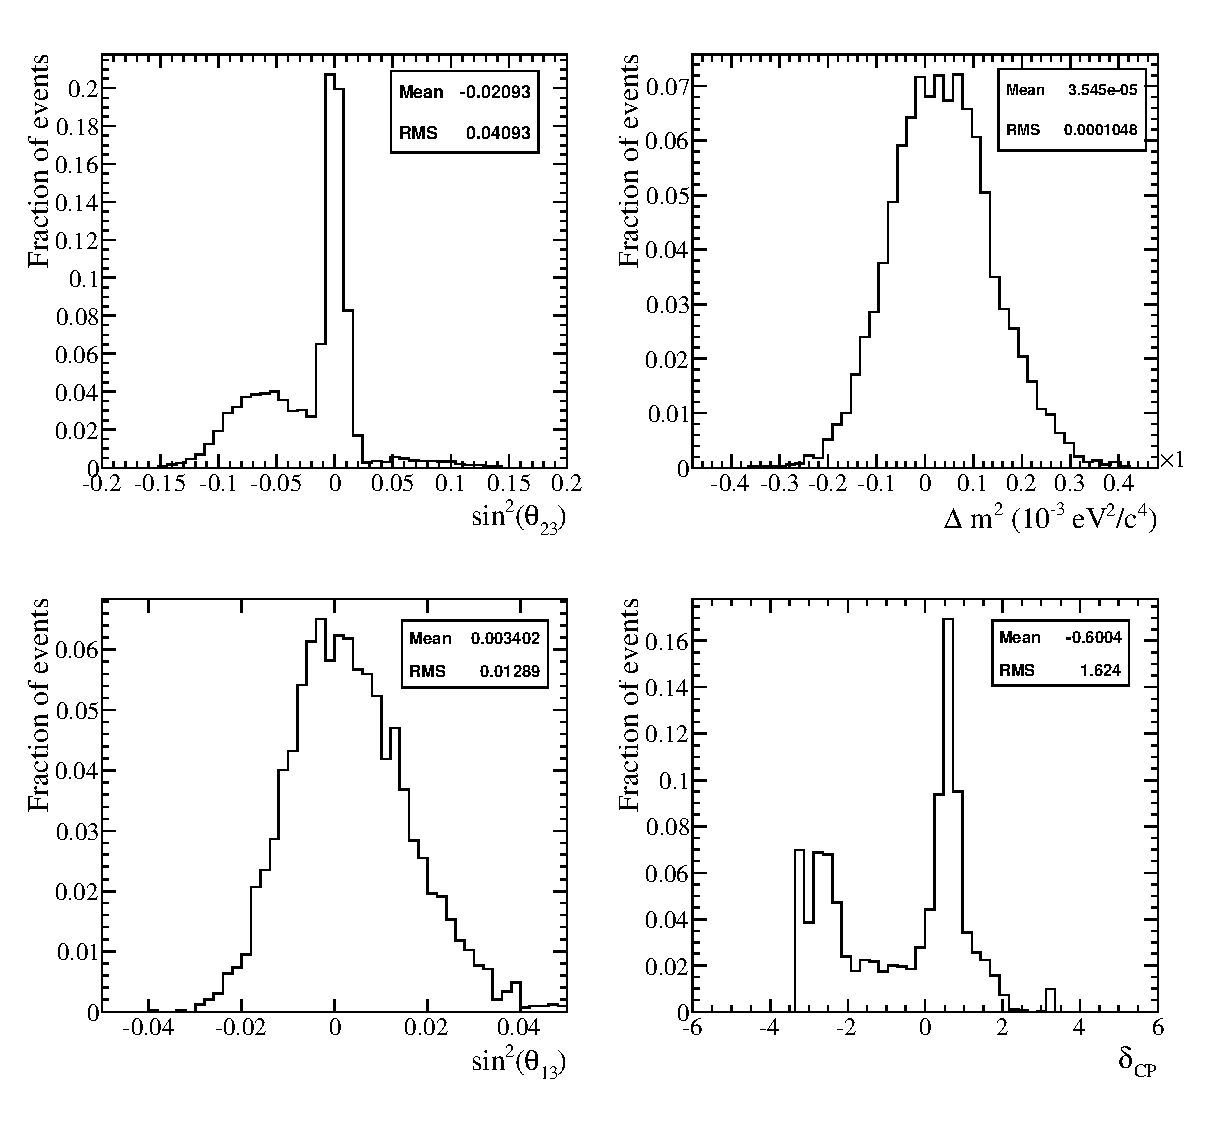
\includegraphics[width=0.7\textwidth]{images/validation/osc_point15_syst.eps}
\caption{Distribution of residuals of the four oscillation parameters at the oscillation point $sin^{2}\theta_{23} = 0.5263$, $sin^{2}\theta_{13} = 0.05$, $\Delta m^{2} = 2.4 \times 10^{-3} eV^{2}/c^{4}$ and $\delta_{CP} = 0$ and normal hierarchy for an ensemble of 5k toy MC experiments. }
\label{fig:validation:residuals}
\end{center}
\end{minipage}
\vfill
\vspace*{0.5cm}
\begin{minipage}[t]{0.75\linewidth}
\begin{center}
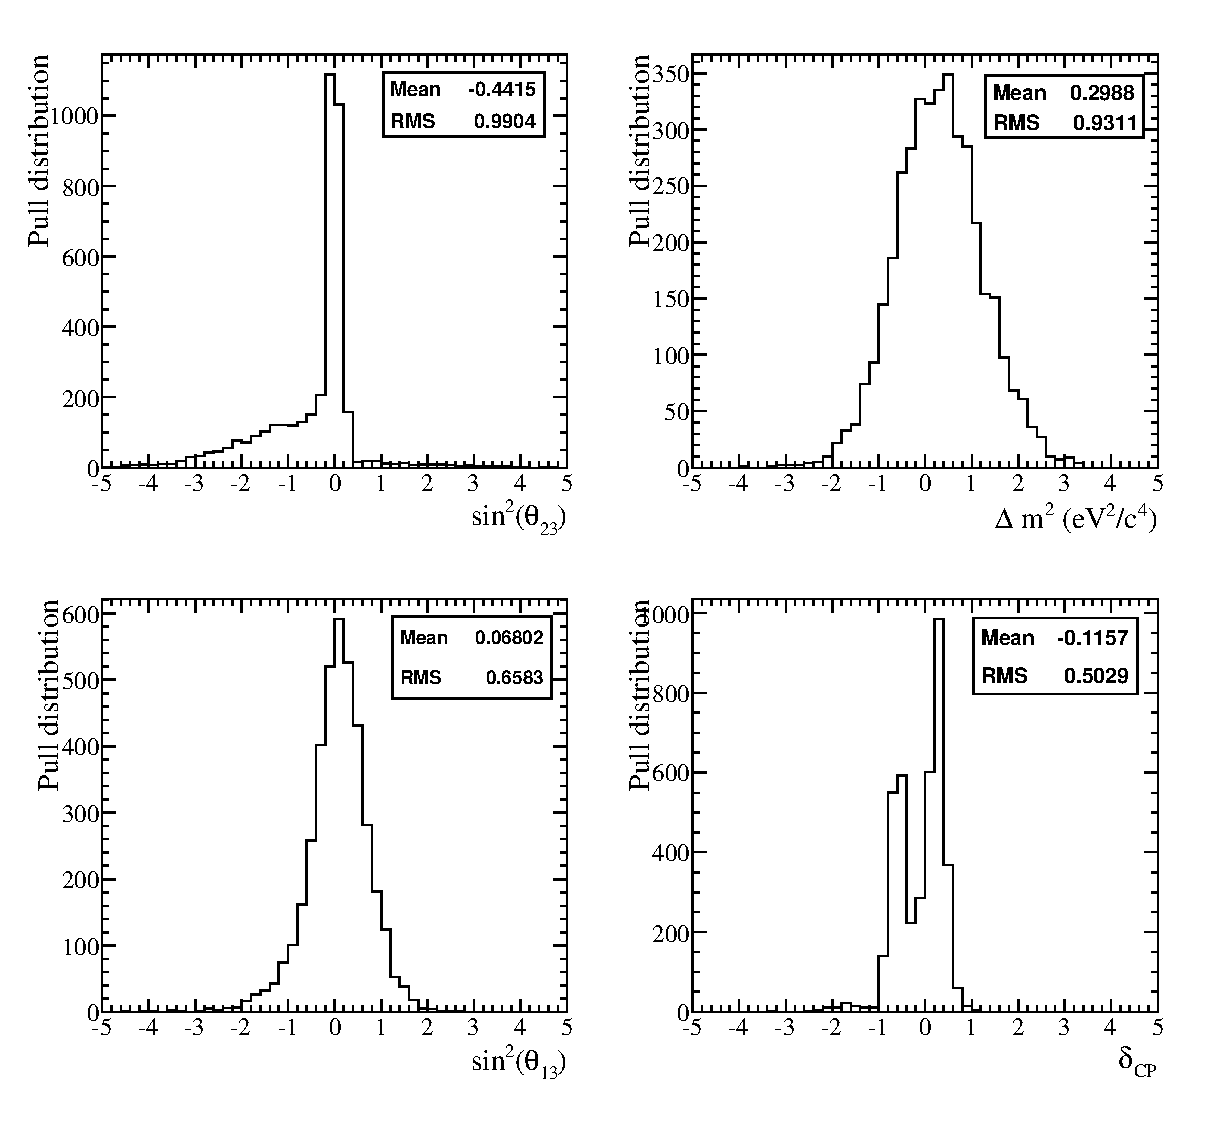
\includegraphics[width=0.7\textwidth]{images/validation/osc_pulls_point15_syst.eps}
\caption{Pulls of the four oscillation parameters at the oscillation point $sin^{2}\theta_{23} = 0.5263$, $sin^{2}\theta_{13} = 0.05$, $\Delta m^{2} = 2.4 \times 10^{-3} eV^{2}/c^{4}$ and $\delta_{CP} = 0$ and normal hierarchy for an ensemble of 5k toy MC experiments. }
\label{fig:validation:pulls}
\end{center}
\end{minipage}
\end{figure}


\begin{figure}[htbp]
\begin{minipage}[t]{0.75\linewidth}
\begin{center}
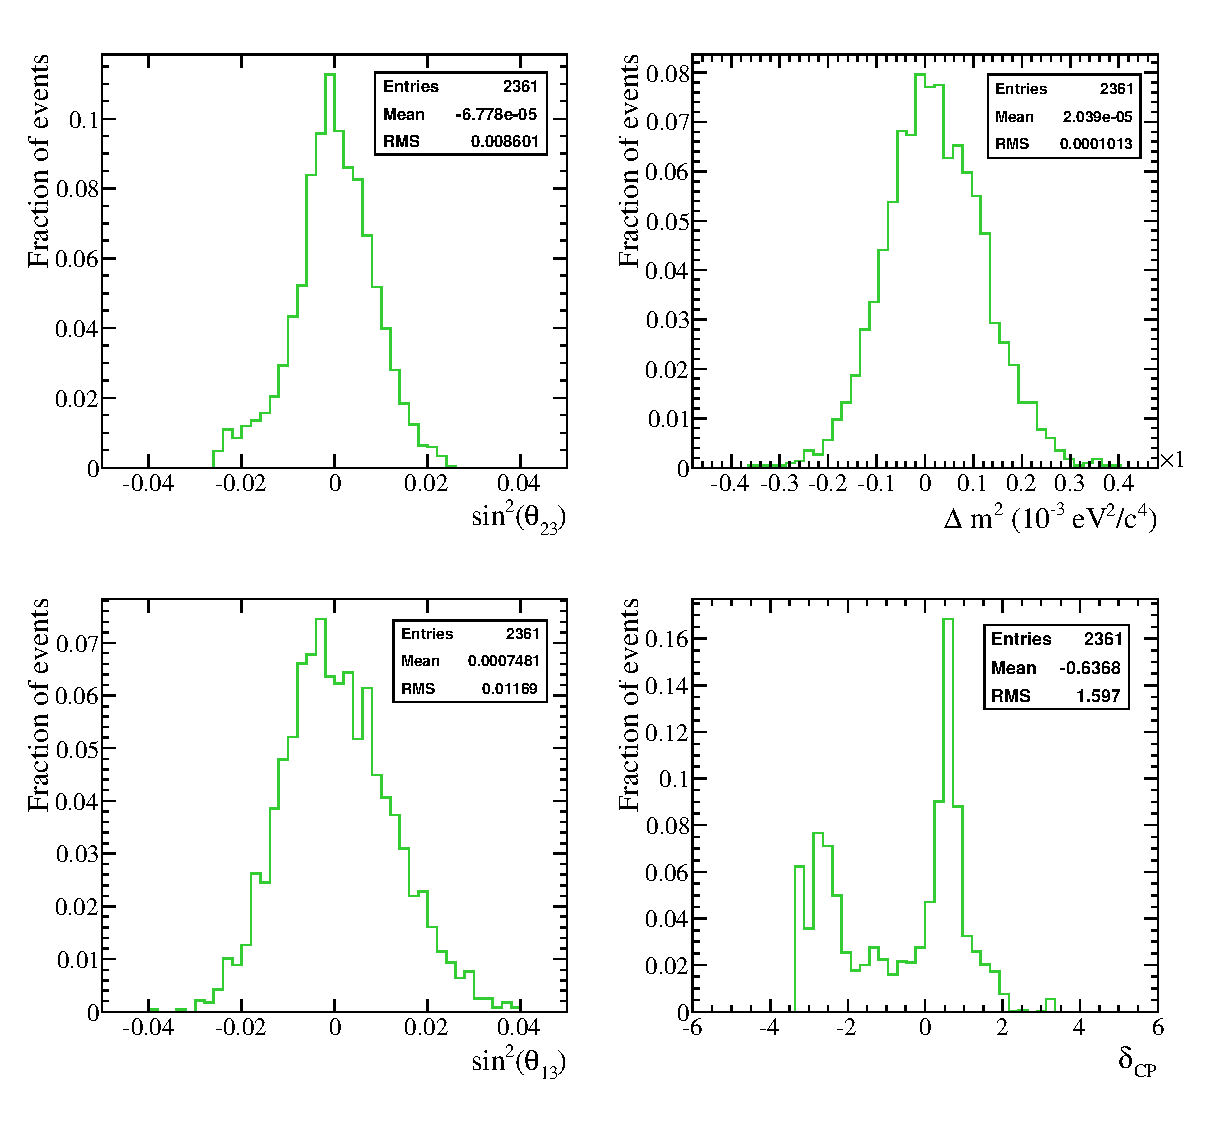
\includegraphics[width=0.7\textwidth]{images/validation/osc_central_point15_syst.eps}
\caption{Distribution of residuals of the four oscillation parameters at the oscillation point $sin^{2}\theta_{23} = 0.5263$, $sin^{2}\theta_{13} = 0.05$, $\Delta m^{2} = 2.4 \times 10^{-3} eV^{2}/c^{4}$ and $\delta_{CP} = 0$ and normal hierarchy for an ensemble of 5k toy MC experiments selecting only those experiments with a best-fit value of $sin^{2}\theta_{23} $ in the central peak. }
\label{fig:validation:residuals_central}
\end{center}
\end{minipage}
\vfill
\vspace*{0.5cm}
\begin{minipage}[t]{0.75\linewidth}
\begin{center}
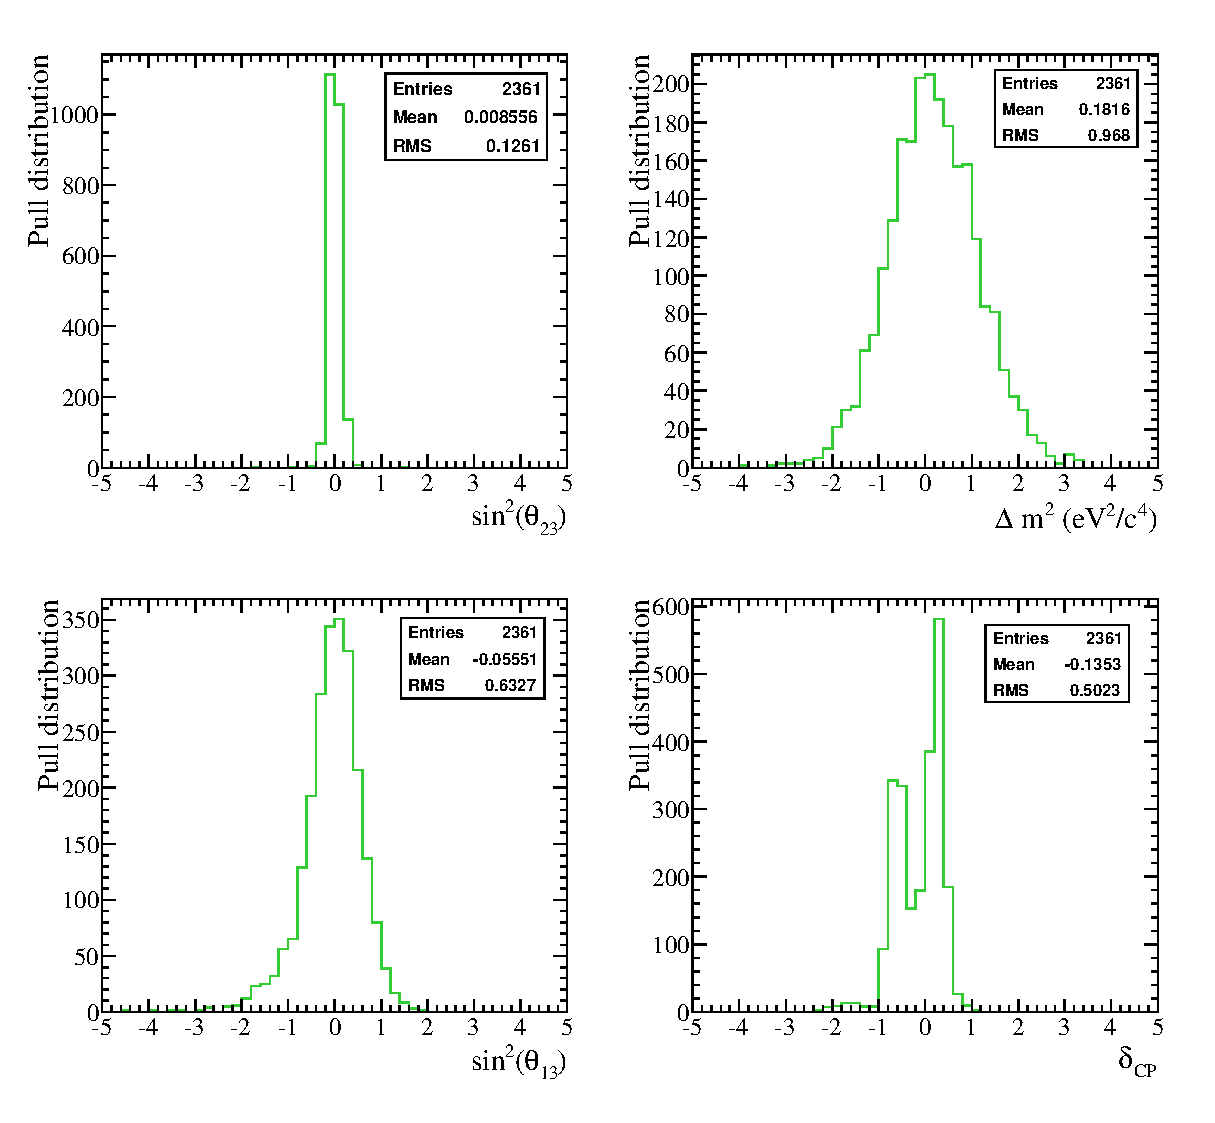
\includegraphics[width=0.7\textwidth]{images/validation/osc_pulls_central_point15_syst.eps}
\caption{Pulls of the four oscillation parameters at the oscillation point $sin^{2}\theta_{23} = 0.5263$, $sin^{2}\theta_{13} = 0.05$, $\Delta m^{2} = 2.4 \times 10^{-3} eV^{2}/c^{4}$ and $\delta_{CP} = 0$ and normal hierarchy for an ensemble of 5k toy MC experiments selecting only those experiments with a best-fit value of $sin^{2}\theta_{23} $ in the central peak.  }
\label{fig:validation:pulls_central}
\end{center}
\end{minipage}
\end{figure}

\begin{figure}[htbp]
\begin{minipage}[t]{0.75\linewidth}
\begin{center}
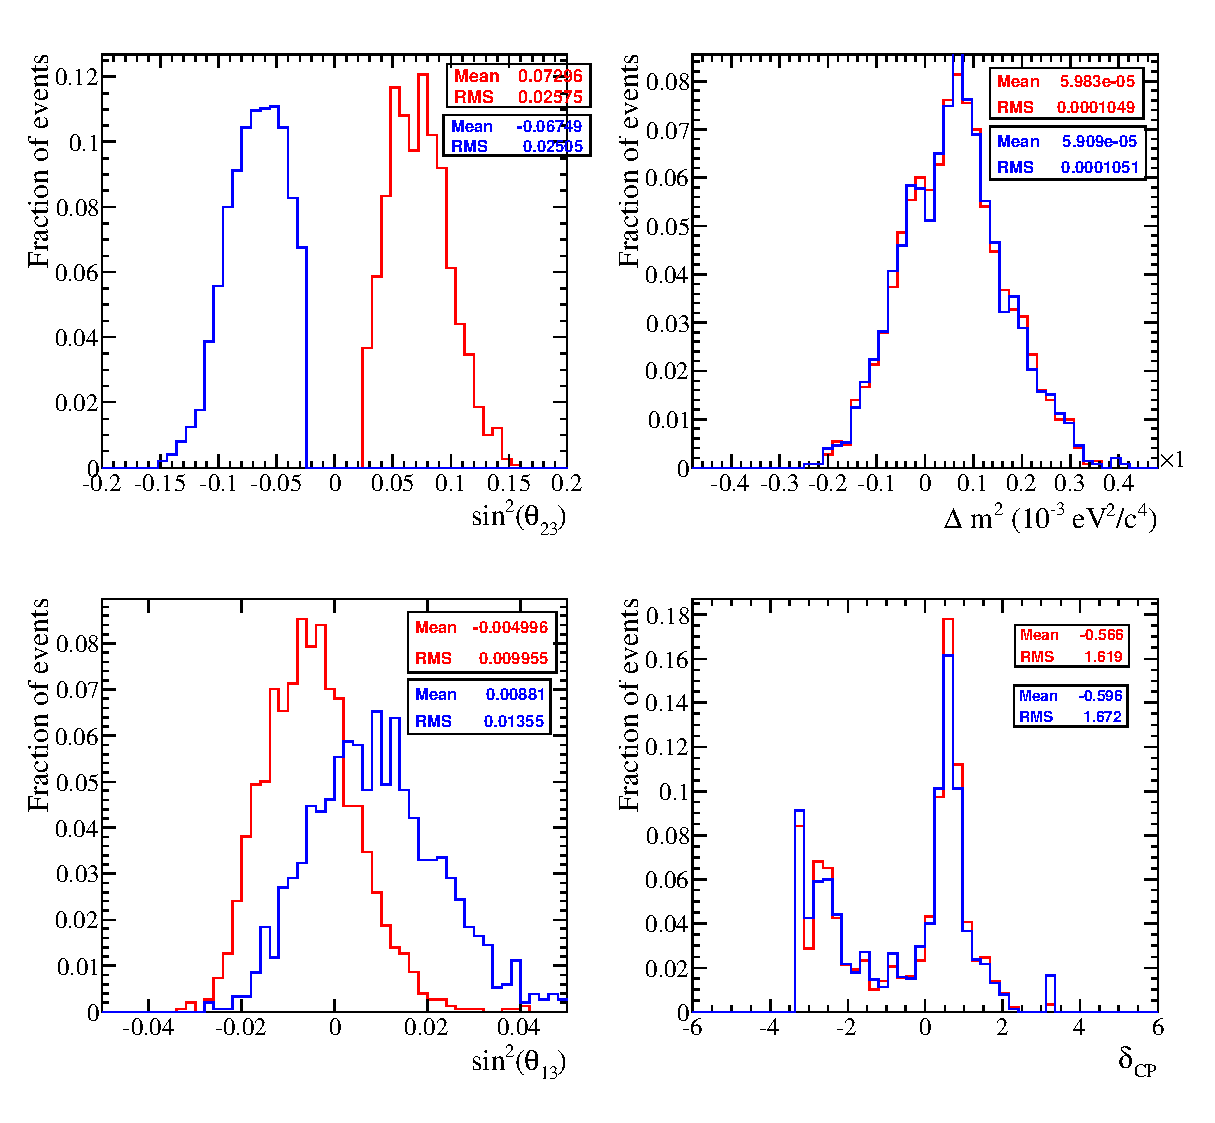
\includegraphics[width=0.7\textwidth]{images/validation/osc_peaks_point15_syst.eps}
\caption{Distribution of residuals of the four oscillation parameters at the oscillation point $sin^{2}\theta_{23} = 0.5263$, $sin^{2}\theta_{13} = 0.05$, $\Delta m^{2} = 2.4 \times 10^{-3} eV^{2}/c^{4}$ and $\delta_{CP} = 0$ and normal hierarchy for an ensemble of 5k toy MC experiments selecting only those experiments with a best-fit value of $sin^{2}\theta_{23} $ in the  peaks away from the true value. Since one of the two peaks is reduced in the joint fit, these figures show the distributions from the two independent fist performed with an initial value in each octant, before selecting the one with minimal $\chi^{2}$. }
\label{fig:validation:residuals_peaks}
\end{center}
\end{minipage}
\vfill
\vspace*{0.5cm}
\begin{minipage}[t]{0.75\linewidth}
\begin{center}
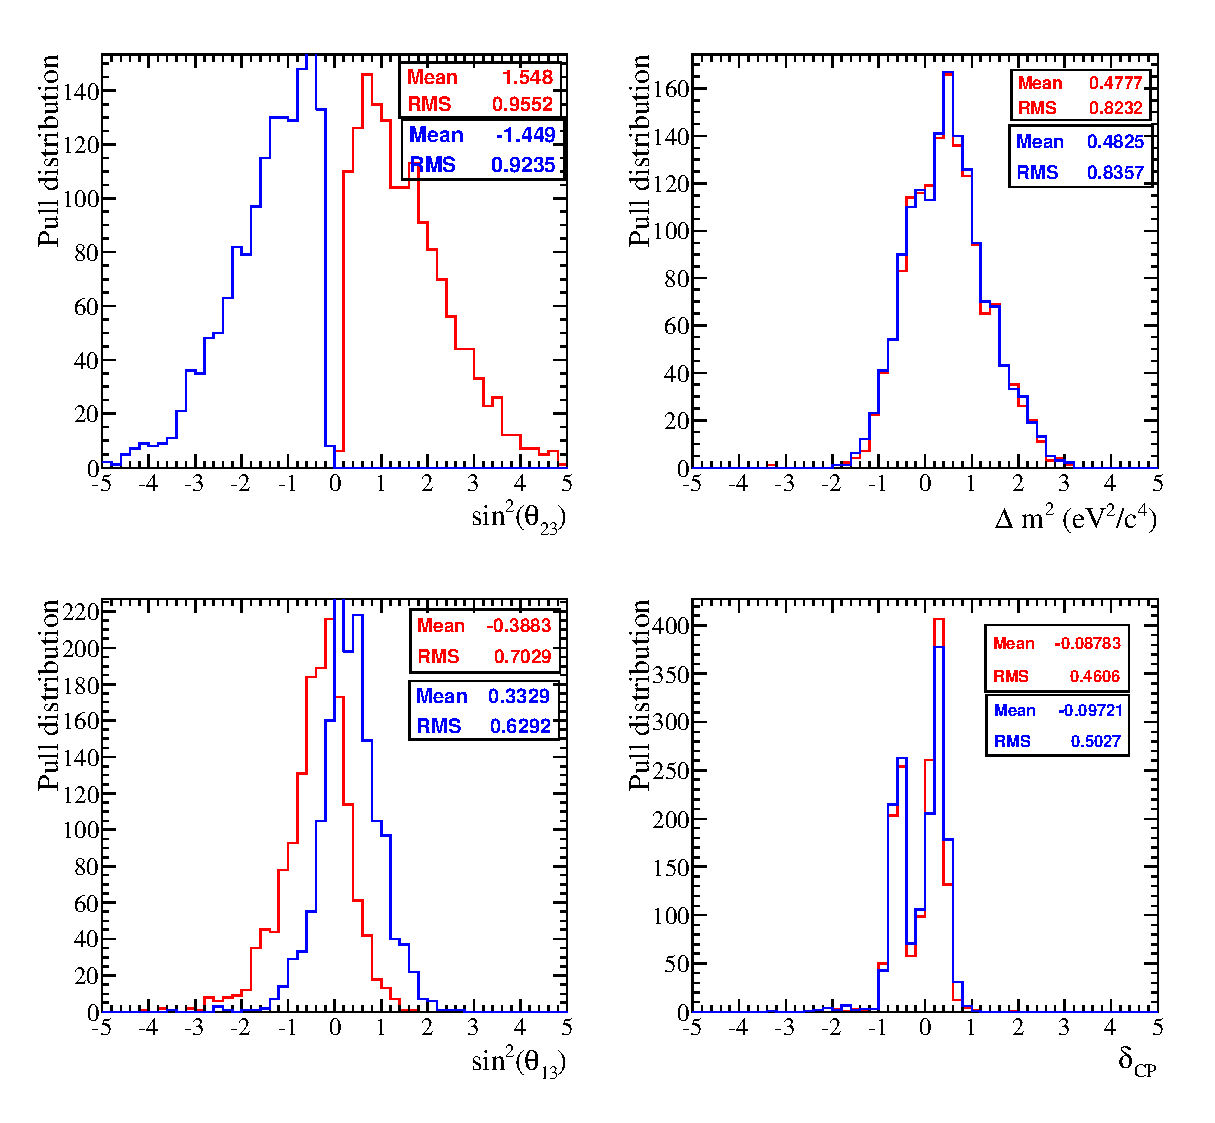
\includegraphics[width=0.7\textwidth]{images/validation/osc_pulls_peaks_point15_syst.eps}
\caption{Pulls of the four oscillation parameters at the oscillation point $sin^{2}\theta_{23} = 0.5263$, $sin^{2}\theta_{13} = 0.05$, $\Delta m^{2} = 2.4 \times 10^{-3} eV^{2}/c^{4}$ and $\delta_{CP} = 0$ and normal hierarchy for an ensemble of 5k toy MC experiments selecting only those experiments with a best-fit value of $sin^{2}\theta_{23} $ in the peaks away from the true value. Since one of the two peaks is reduced in the joint fit, these figures show the distributions from the two independent fist performed with an initial value in each octant, before selecting the one with minimal $\chi^{2}$.  }
\label{fig:validation:pulls_peaks}
\end{center}
\end{minipage}
\end{figure}


\begin{figure}[htbp]
\begin{minipage}[t]{0.75\linewidth}
\begin{center}
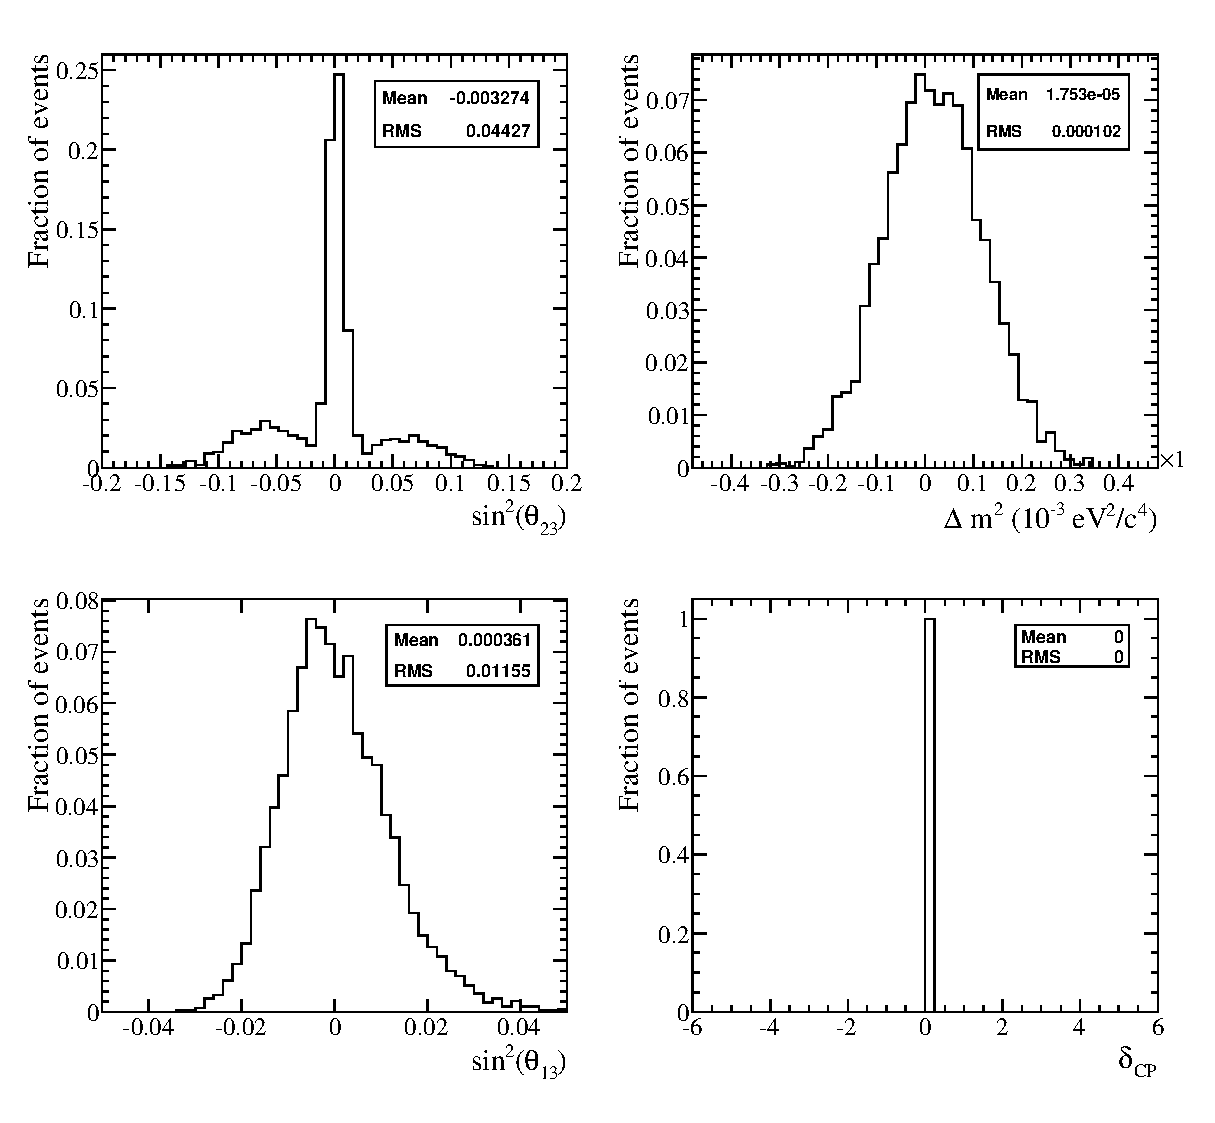
\includegraphics[width=0.7\textwidth]{images/validation/osc_point19_syst.eps}
\caption{Distribution of residuals of the four oscillation parameters at the oscillation point $sin^{2}\theta_{23} = 0.5263$, $sin^{2}\theta_{13} = 0.05$, $\Delta m^{2} = 2.4 \times 10^{-3} eV^{2}/c^{4}$ and $\delta_{CP} = 0$ and normal hierarchy for an ensemble of 4k toy MC experiments and fixing $\delta_{CP}$ to its true value. }
\label{fig:validation:residuals_fixdcp}
\end{center}
\end{minipage}
\vfill
\vspace*{0.5cm}
\begin{minipage}[t]{0.75\linewidth}
\begin{center}
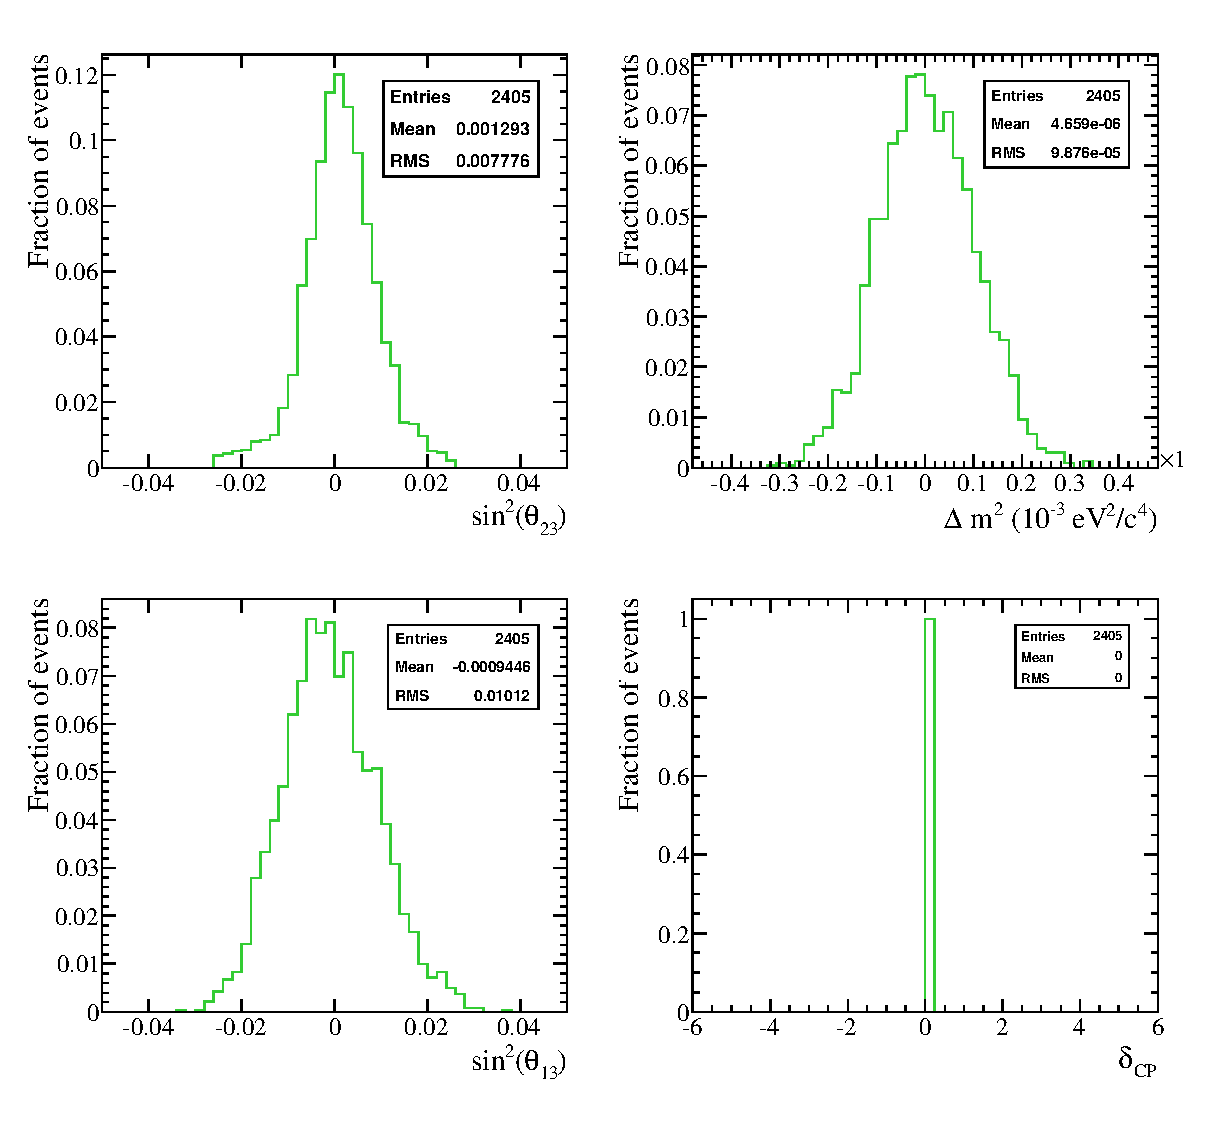
\includegraphics[width=0.7\textwidth]{images/validation/osc_central_point19_syst.eps}
\caption{Distribution of residuals of the four oscillation parameters at the oscillation point $sin^{2}\theta_{23} = 0.5263$, $sin^{2}\theta_{13} = 0.05$, $\Delta m^{2} = 2.4 \times 10^{-3} eV^{2}/c^{4}$ and $\delta_{CP} = 0$ and normal hierarchy for an ensemble of 4k toy MC experiments and fixing $\delta_{CP}$ to its true value, selecting only those experiments with a best-fit value of $sin^{2}\theta_{23} $ in the central peak. }
\label{fig:validation:residuals_central_fixdcp}
\end{center}
\end{minipage}
\end{figure}

\begin{figure}[htbp]
\begin{center}
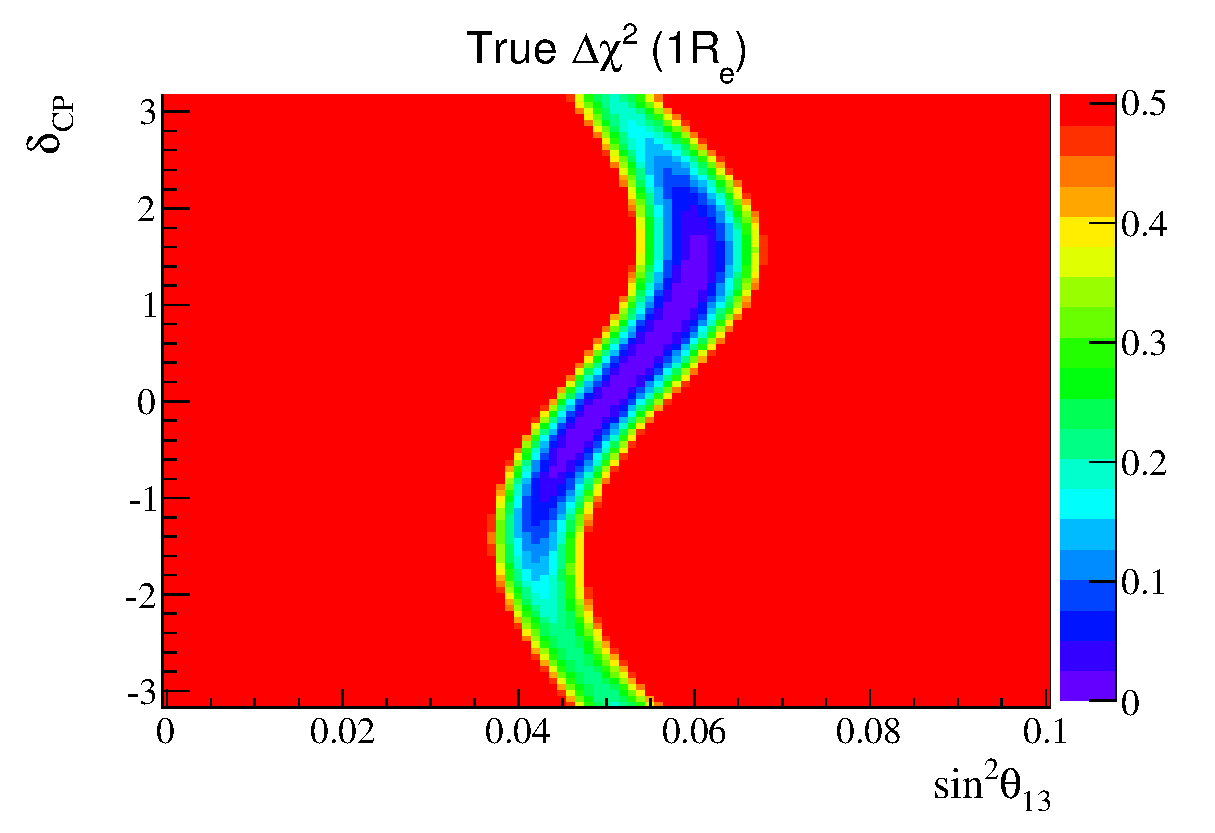
\includegraphics[width=0.7\textwidth]{images/validation/TrueDeltaChisqZoom.eps}
\caption{True $\Delta\chi^{2}$ distribution for the single e-like ring sample in the
($sin^{2}\theta_{13}$,$\delta_{CP}$) space for a toy created at the oscillation point 
$sin^{2}\theta_{23} = 0.5263$, $sin^{2}\theta_{13} = 0.05$, $\Delta m^{2} = 2.4 \times 10^{-3} eV^{2}/c^{4}$ and $\delta_{CP} = 0$
assuming normal hierarchy without statistical fluctuations nor systematic variations.}
\label{fig:validation:truechisq}
\end{center}
\end{figure}

\begin{figure}[htbp]
\begin{center}
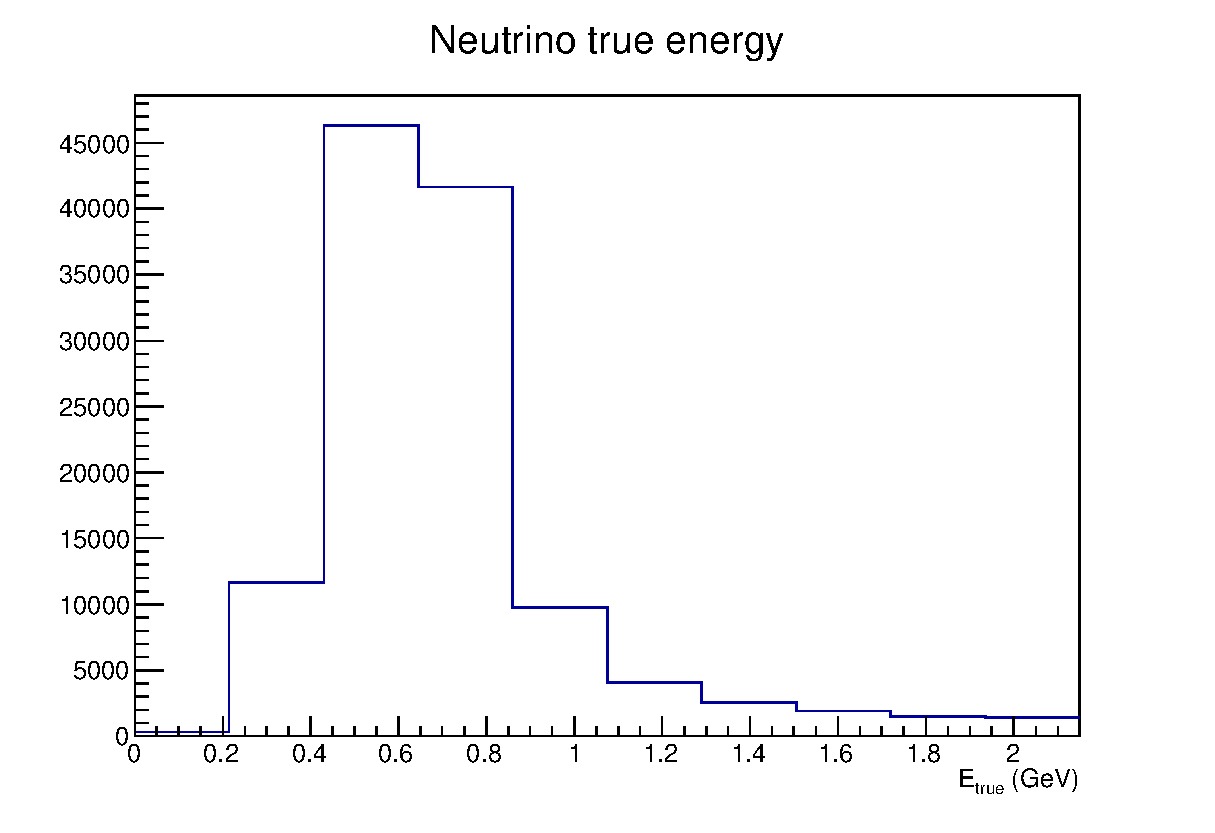
\includegraphics[width=0.5\textwidth]{images/validation/EtrueSigNueEvents.eps}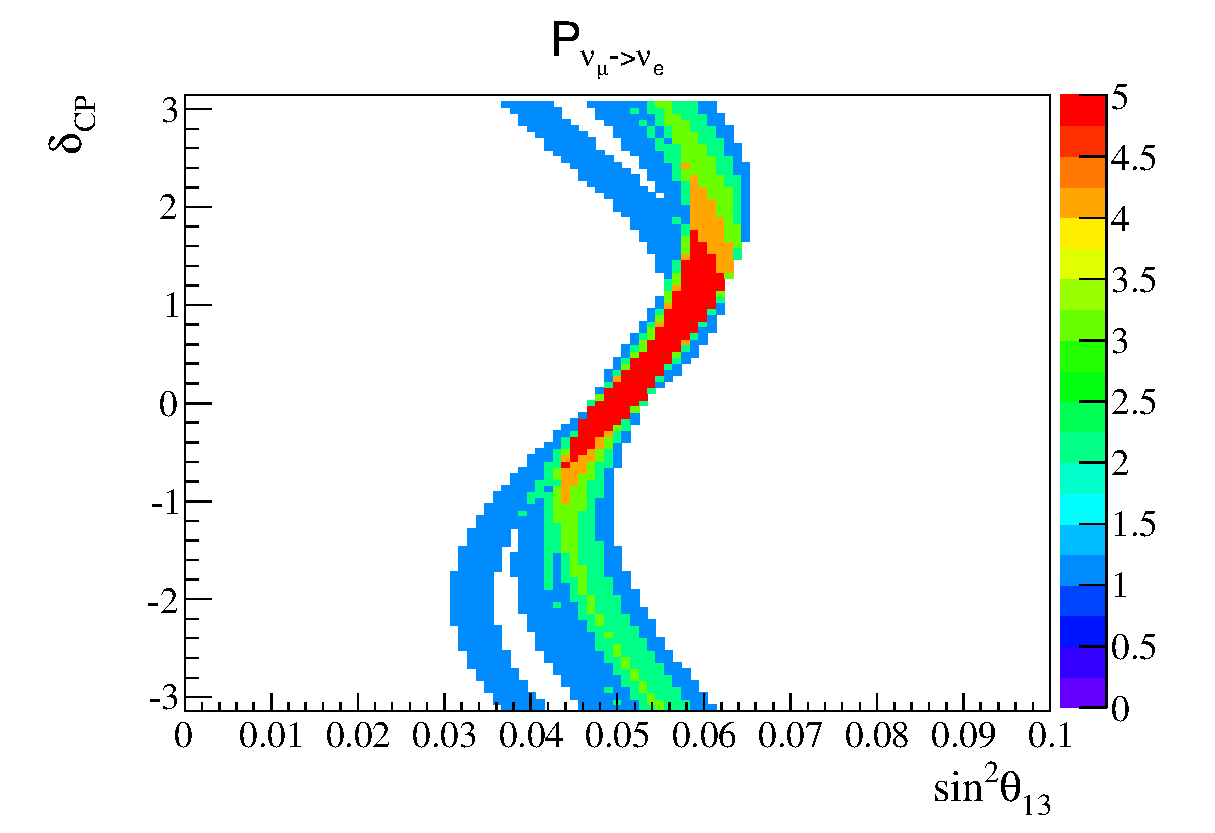
\includegraphics[width=0.5\textwidth]{images/validation/OscProbLines.eps}
\caption{On the left: true energy spectrum for the single e-like ring
event candidates for the oscillated $\nu_{e}$ category in the T2K SKMC, zooming around the peak of the spectrum. On the right:
 lines of equal $P(\nu_{\mu}\rightarrow\nu_{e})$ are drawn for the different values of the true energy
at the peak of the spectrum on the left side (from 0.45 GeV to 0.85 GeV). The $P(\nu_{\mu}\rightarrow\nu_{e})$ to draw these 
lines is selected to be the one corresponding to the oscillation point 
$sin^{2}\theta_{23} = 0.5263$, $sin^{2}\theta_{13} = 0.05$, $\Delta m^{2} = 2.4 \times 10^{-3} eV^{2}/c^{4}$ and $\delta_{CP} = 0$
(in a range of $\Delta(P(\nu_{\mu}\rightarrow\nu_{e})) < 0.005$).}
\label{fig:validation:biasdeltacp}
\end{center}
\end{figure}

\begin{figure}[htbp]
\begin{center}
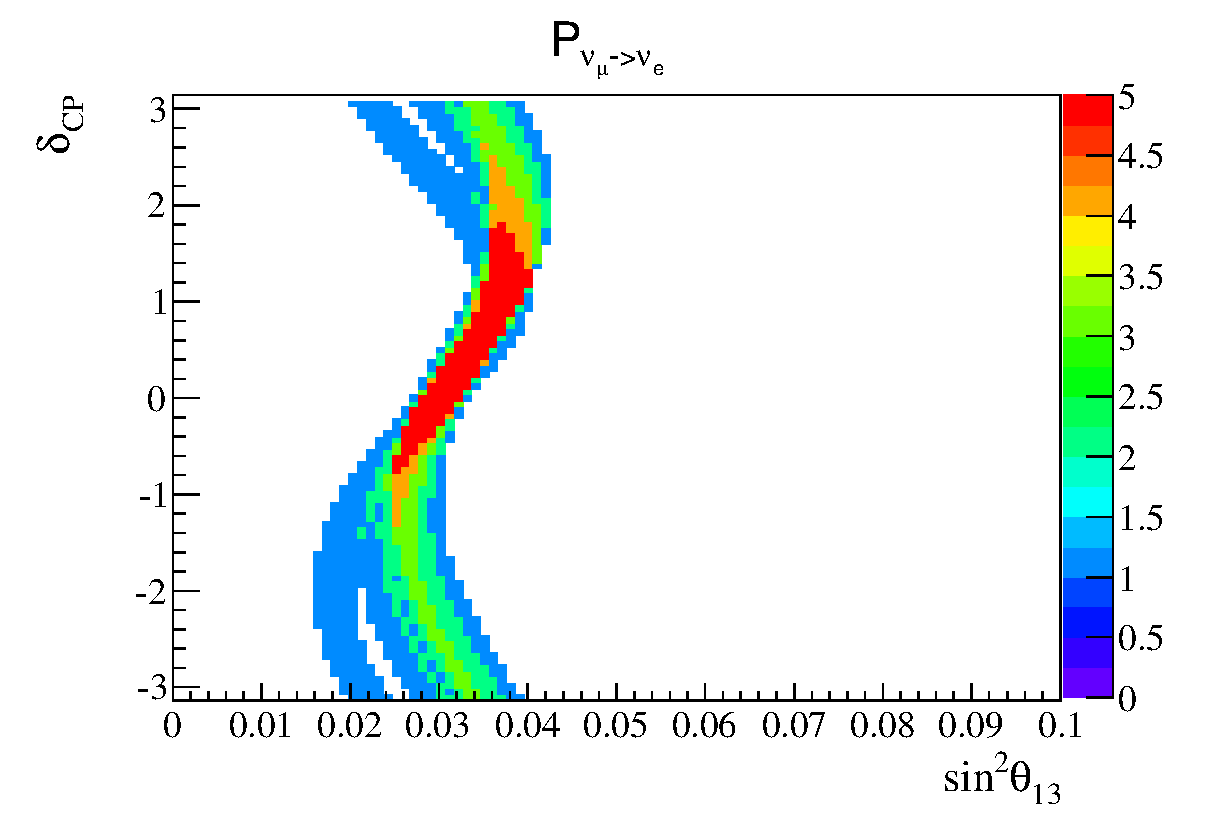
\includegraphics[width=0.5\textwidth]{images/validation/OscProbLinesChangedTheta13.eps}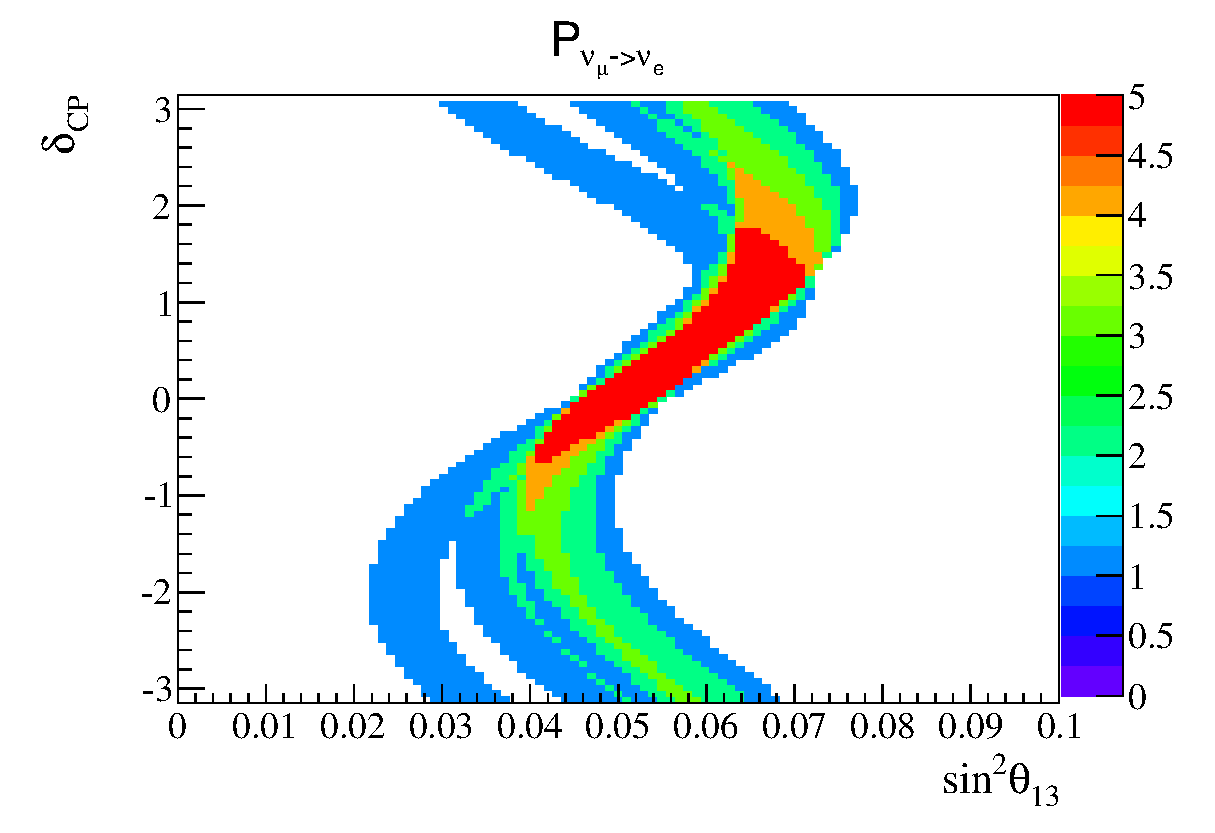
\includegraphics[width=0.5\textwidth]{images/validation/OscProbLinesChangedTheta23.eps}
\caption{Lines of equal $P(\nu_{\mu}\rightarrow\nu_{e})$ are drawn for the different values of the true energy
at the peak of the spectrum on the left side of Fig. \ref{fig:validation:biasdeltacp} (from 0.45 GeV to 0.85 GeV)
corresponding to the oscillation point $sin^{2}\theta_{23} = 0.5263$, $sin^{2}\theta_{13} = 0.03$, $\Delta m^{2} = 2.4 \times 10^{-3} eV^{2}/c^{4}$ and $\delta_{CP} = 0$ (left) and
$sin^{2}\theta_{23} = 0.3$, $sin^{2}\theta_{13} = 0.05$, $\Delta m^{2} = 2.4 \times 10^{-3} eV^{2}/c^{4}$ and $\delta_{CP} = 0$ (right).
}
\label{fig:validation:biasdeltacp2}
\end{center}
\end{figure}

\begin{figure}[htbp]
\begin{center}
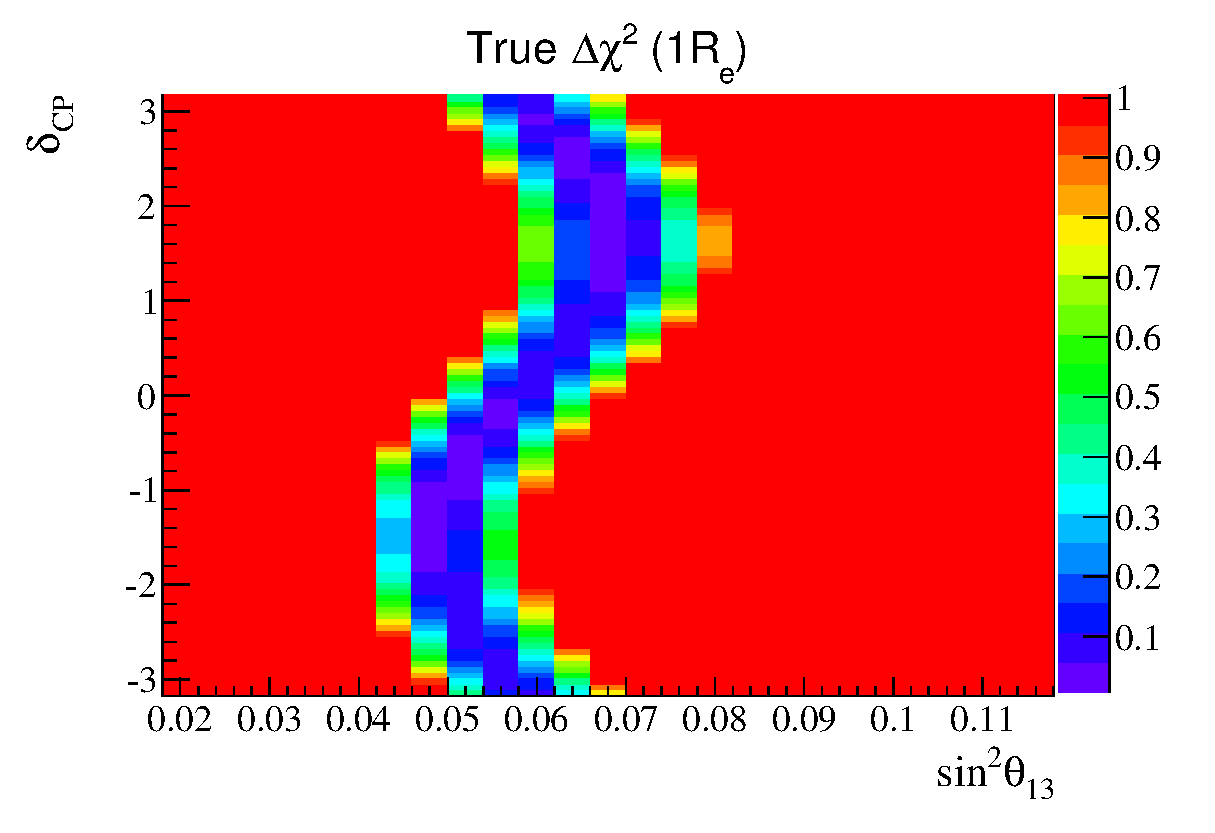
\includegraphics[width=0.5\textwidth]{images/validation/TrueDeltaChisqZoomNegativeDelta.eps}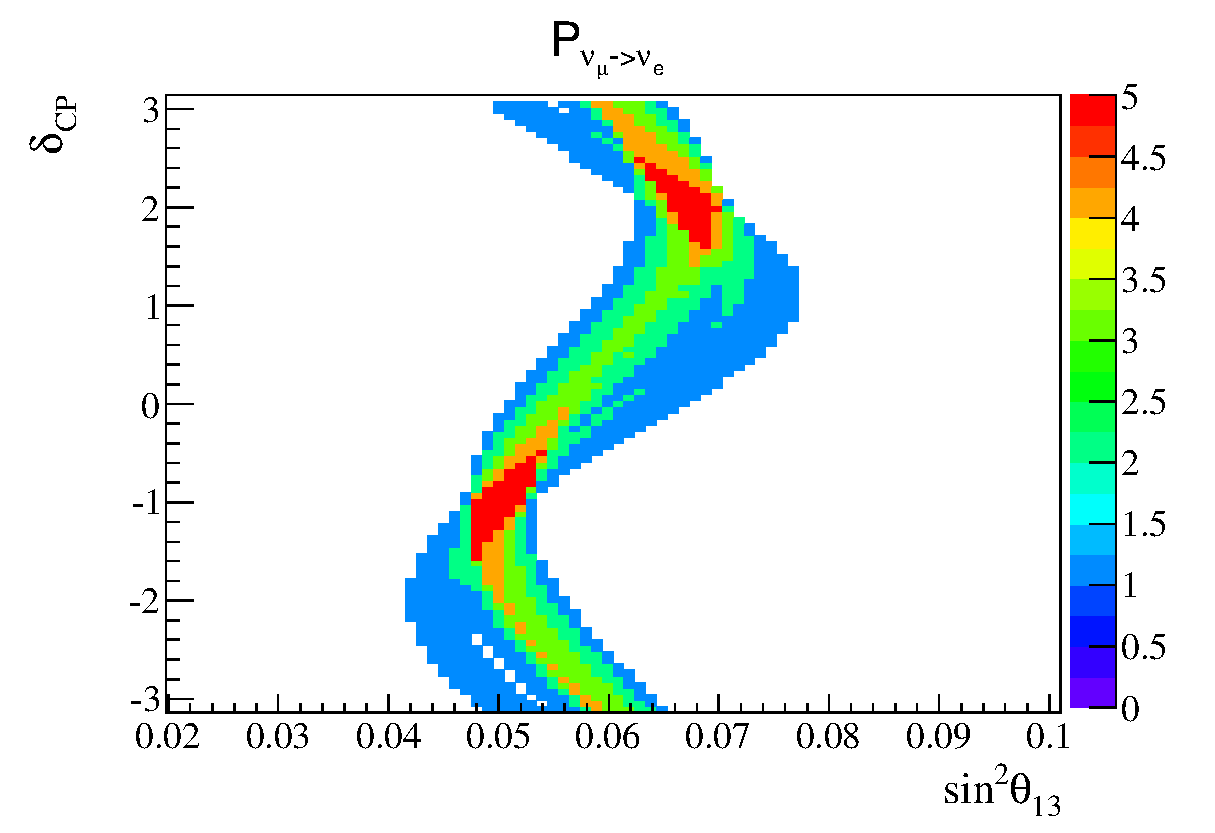
\includegraphics[width=0.5\textwidth]{images/validation/OscProbLinesNegativeDelta.eps}
\caption{On the left: true $\Delta\chi^{2}$ distribution for the single e-like ring sample in the
($sin^{2}\theta_{13}$,$\delta_{CP}$) space for a toy created at the oscillation point 
$sin^{2}\theta_{23} = 0.5263$, $sin^{2}\theta_{13} = 0.05$, $\Delta m^{2} = 2.4 \times 10^{-3} eV^{2}/c^{4}$ and $\delta_{CP} = -1$
assuming normal hierarchy without statistical fluctuations nor systematic variations. On the right: lines of equal $P(\nu_{\mu}\rightarrow\nu_{e})$ are drawn for the different values of the true energy at the peak of the spectrum on the left side of Fig. \ref{fig:validation:biasdeltacp} (from 0.45 GeV to 0.85 GeV)
corresponding to the oscillation point $sin^{2}\theta_{23} = 0.5263$, $sin^{2}\theta_{13} = 0.03$, $\Delta m^{2} = 2.4 \times 10^{-3} eV^{2}/c^{4}$ and $\delta_{CP} = -1$.
}
\label{fig:validation:biasdeltacp3}
\end{center}
\end{figure}







\clearpage
\subsection{Residuals and pulls for the systematic parameters}

Distributions of pulls of the 64 systematic parameters are presented in Figs. \ref{fig:validation:pulls1}-\ref{fig:validation:pulls7} for an oscillation point with $sin^{2}\theta_{23} = 0.513$, $sin^{2}\theta_{13} = 0.0251$, $\Delta m^{2} = 2.4 \times 10^{-3} eV^{2}/c^{4}$ and $\delta_{CP} = 0$ including correlations between the SK efficiencies for the two samples. A summary of the pull mean and RMS is given in Fig. \ref{fig:validation:summary} comparing results with and without correlations. From this figure it is clear that only small changes appear when introducing the correlations between the SK efficiencies for the two samples.

No problems were identified in the tests done to the fitter, which performed as expected.
In general all systematic parameters present a good behaviour with a mean in $\approx 0$ and RMS $\approx 1$. 
There are some small biases in the pull distributions for some systematic parameters, which are understood: 

\begin{itemize}
\item{\textbf{Spectral function}

A special treatment is followed for this parameter, which is varied following a Gaussian distribution bounded between [0,1] when creating toy experiments
and when fitting this parameter is limited to the same range [0,1] and a Gaussian constraint in the penalty term is applied. Therefore, a Gaussian distribution of residuals
centered at 0 with RMS 1 is not expected for this parameter.
}

\item{\textbf{$\pi$-less $\Delta$ decay}

The distribution of pulls for this parameter appears to be biased due to the special procedure followed to calculate the weights for the response functions (splines) for this parameter. 
In NEUT, 20\% of the $\Delta$s decay within this process, being therefore the uncertainty equal to 20\%. That means that this parameter cannot be tweaked to values smaller than -1$\sigma$, what would be unphysical, and instead the same weight found for a tweak of -1$\sigma$ is applied to any tweak smaller that this value, creating an assymmetry and a constant plateau at negative values. Thus, a small negative bias appears for this parameter.
}

\item{\textbf{SuperK reconstructed energy scale}

This systematic is different from the others since its effect is not translated into a weight of the number of events in a bin, but a migration of events from one bin to the adjacent ones. 
The single $\mu$-like ring spectrum is not symmetric and therefore a positive tweak of the reconstructed energy scale parameter has a different effect in the spectrum than a negative one as already explained in the \textit{VALOR} Run1+2+3+4 $\nu_{\mu}$ disappearance analysis in \cite{OurRun1234DisappAnalysis3Flavour}. There is also an asymmetric effect in the single e-like ring spectrum, more evident in the first and last bins (as can be seen in  Fig. 46 in the additional material accompanying this technical note \cite{AdditionalMaterial}). The RMS of this parameter is larger than 1, issue that can be solved if MINOS errors are computed instead of the ones calculated with the HESSE algorithm, since MINOS errors are different for positive and negative values of the distribution of residuals and they therefore account for the asymmetric effect of this parameter. %In Fig. \ref{fig:validation:summary} the value of the RMS from the pull distribution calculated with MINOS errors for this systematic parameter is drawn as a green point.
}

\item{\textbf{$1R_{\mu}$ NC SK efficiency + FSI + SI}

There distribution of pulls for this parameter is biased to a negative value due to the low statistics at current POT, which makes that a downward Poisson fluctuation of the small number of events in the bins around the oscillation dip in the single $\mu$-like ring spectrum is more likely than an upward fluctuation. Since NC events are mainly distributed around the oscillation dip, and downward fluctuations are more likely to happen in that zone of the spectrum, then a movement to a smaller value of this systematic parameter is more probable and creates a bias to negative values, which disappears when increasing the POT and the number of events at the oscillation dip, reducing the predominance of downward fluctuations.
}


%\item{\textbf{$1R_{e}$ $\nu_{\mu}$ CC SK efficiencies + FSI + SI}

%{\color{red}{These parameters are not biased, but their RMS is smaller than 1 ($\approx. 0.8), what means that the error %returned by the fitter is overestimated, quite likely due to the fact that their fractional error is $\approx 1.2$ ... }}

%}

\end{itemize}


\begin{figure}[htbp]
\begin{center}
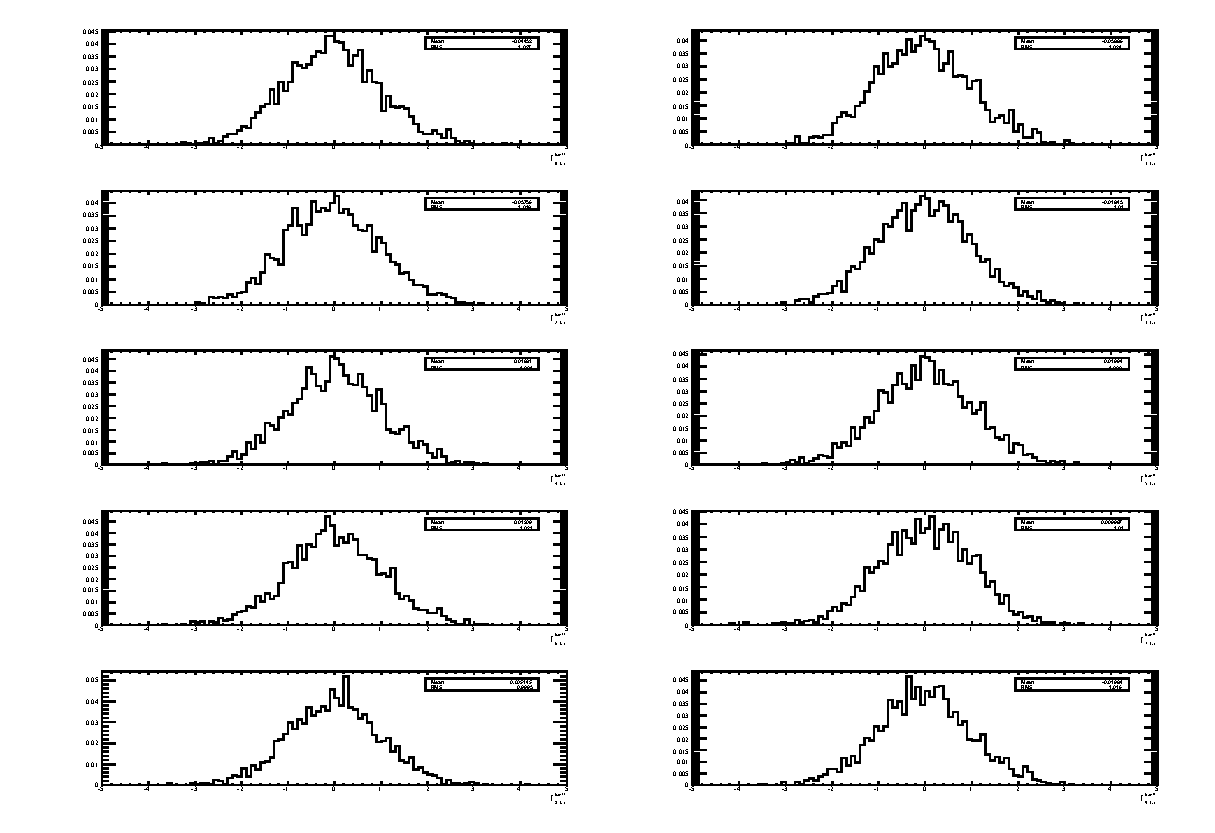
\includegraphics[width=1.0\textwidth]{images/validation/joint_pulls_point0_new_corr_hesse_pull_all_1.eps}
\caption{Distribution of pulls for the systematic parameters BANFF 0 - 9.
}
\label{fig:validation:pulls1}
\end{center}
\end{figure}



\begin{figure}[htbp]
\begin{center}
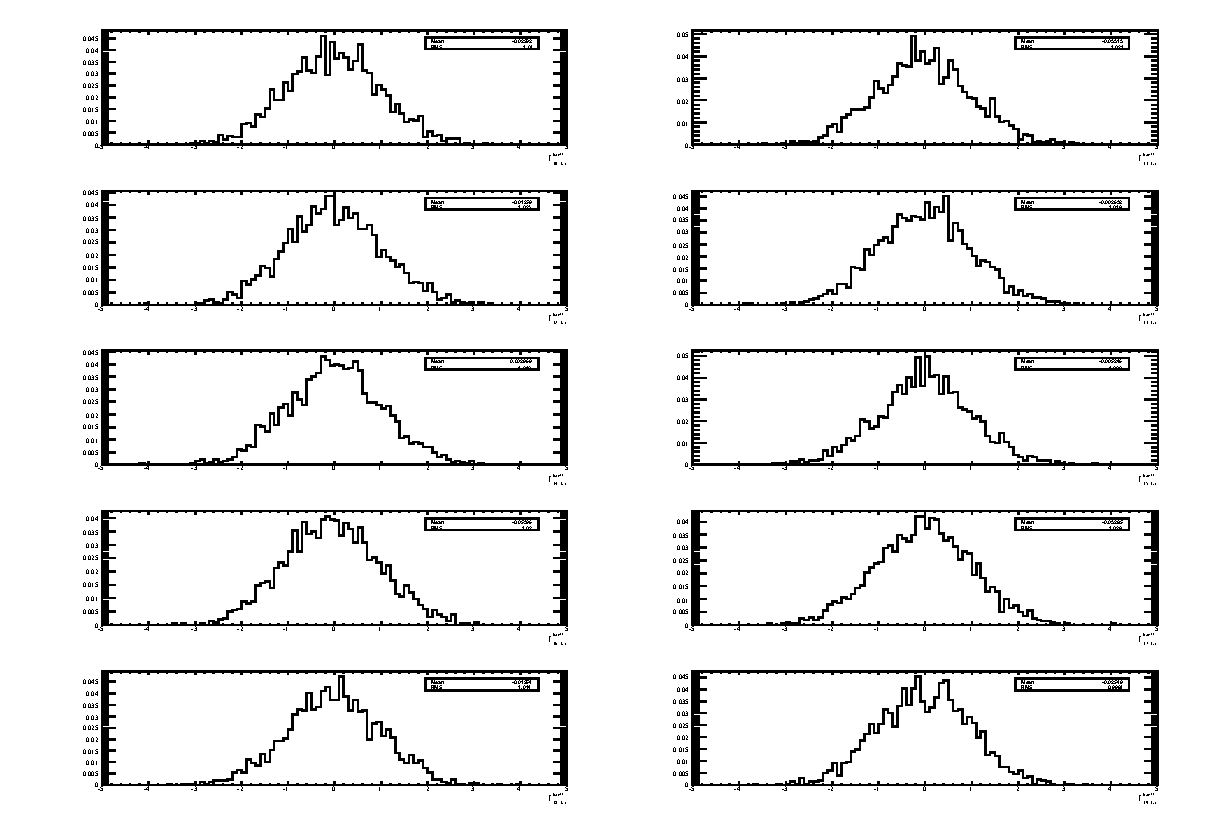
\includegraphics[width=1.0\textwidth]{images/validation/joint_pulls_point0_new_corr_hesse_pull_all_2.eps}
\caption{Distribution of pulls for the systematic parameters BANFF 10 - 19.
}
\label{fig:validation:pulls2}
\end{center}
\end{figure}

\begin{figure}[htbp]
\begin{center}
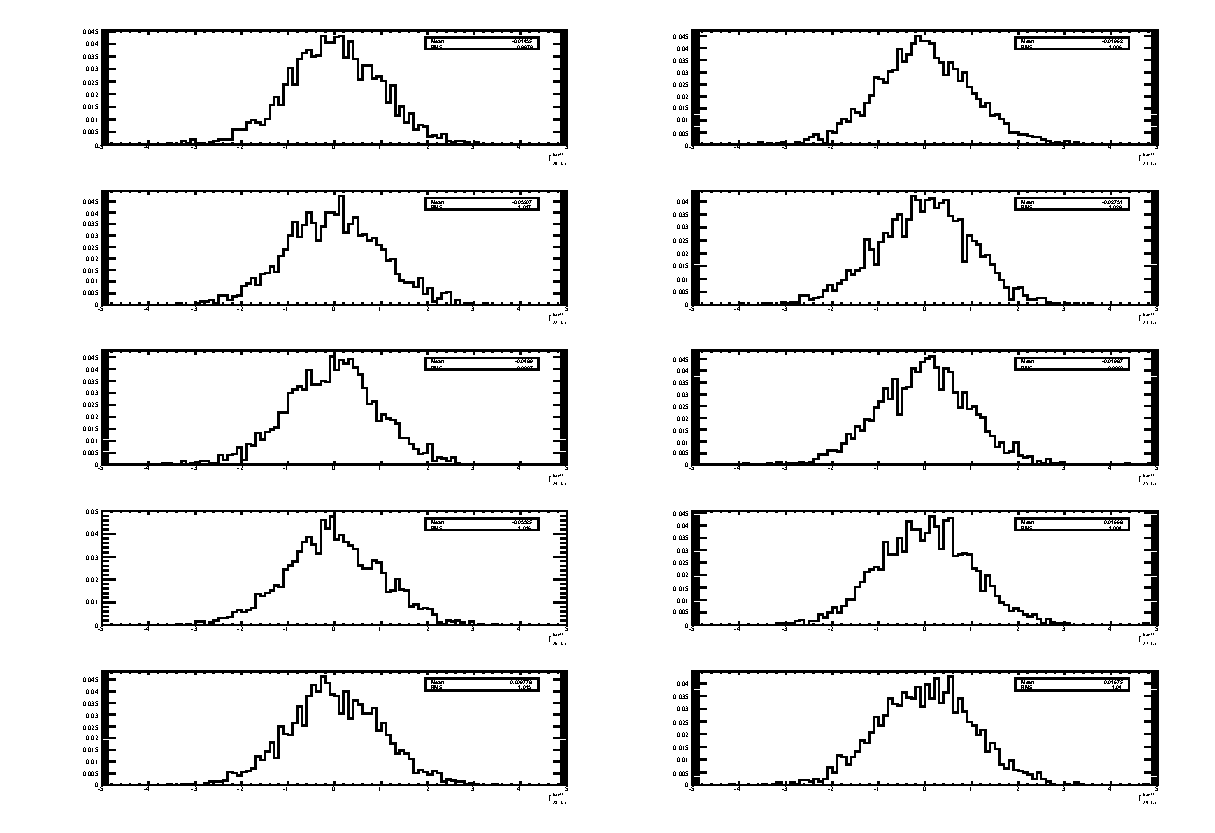
\includegraphics[width=1.0\textwidth]{images/validation/joint_pulls_point0_new_corr_hesse_pull_all_3.eps}
\caption{Distribution of pulls for the systematic parameters BANFF  20 - 29.
}
\label{fig:validation:pulls3}
\end{center}
\end{figure}

\begin{figure}[htbp]
\begin{center}
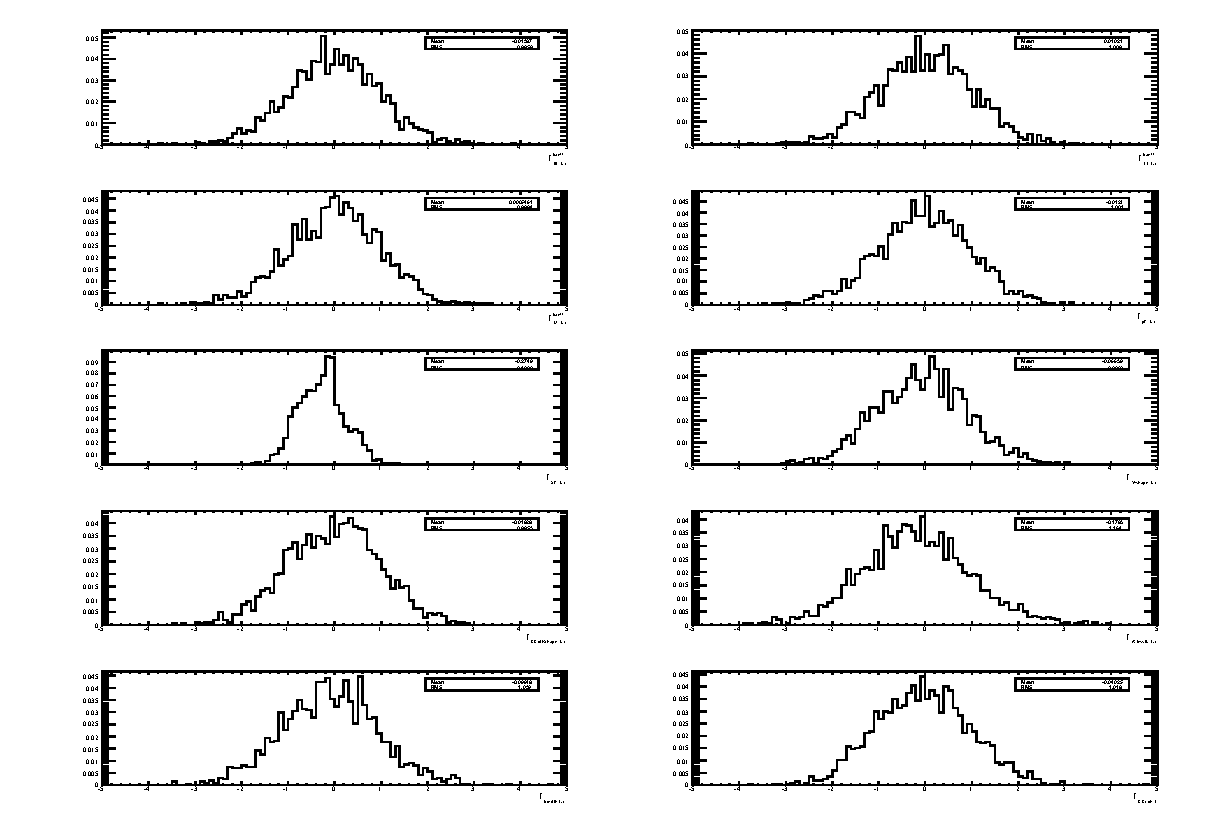
\includegraphics[width=1.0\textwidth]{images/validation/joint_pulls_point0_new_corr_hesse_pull_all_4.eps}
\caption{Distribution of pulls for the systematic parameters BANFF 30 - 32 and some of the uncorrelated cross section systematics.
}
\label{fig:validation:pulls4}
\end{center}
\end{figure}

\begin{figure}[htbp]
\begin{center}
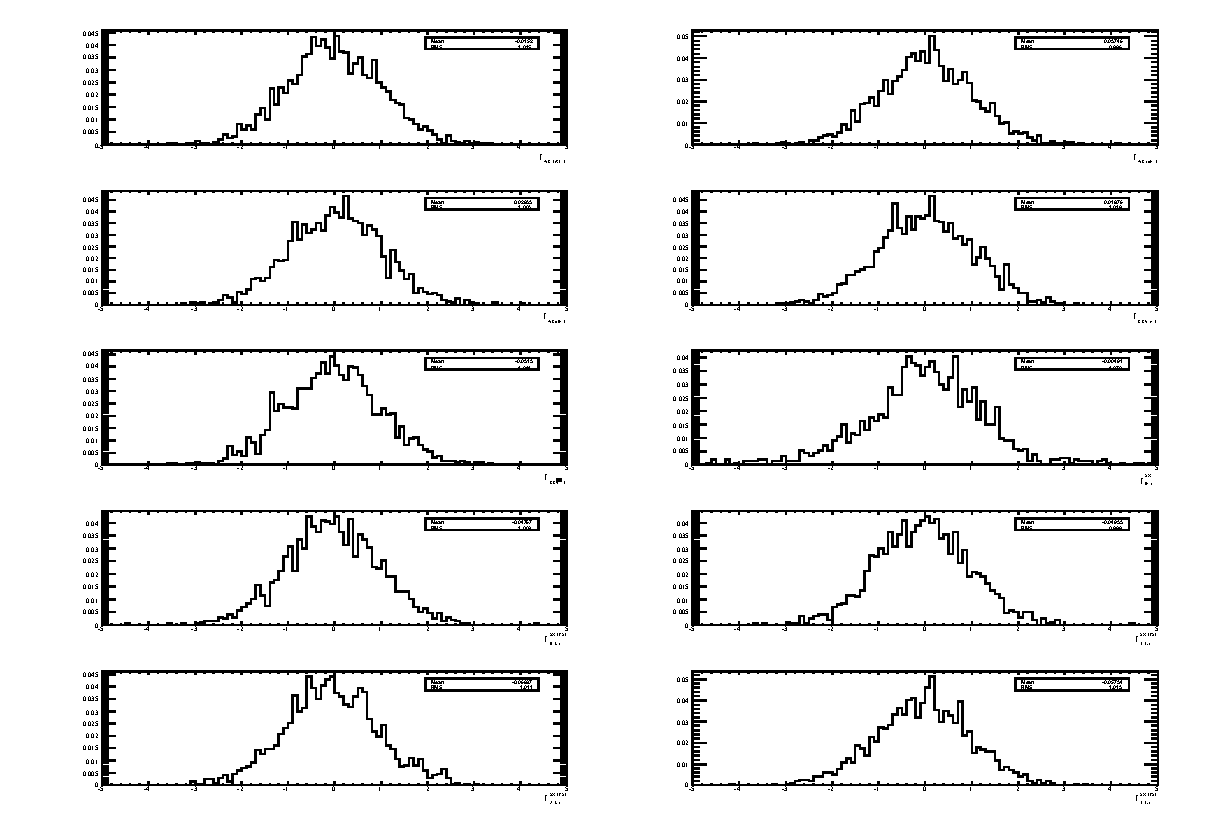
\includegraphics[width=1.0\textwidth]{images/validation/joint_pulls_point0_new_corr_hesse_pull_all_5.eps}
\caption{Distribution of pulls for some of the uncorrelated cross section systematics, reconstructed Energy scale and SK+FSI parameters 0-3.
}
\label{fig:validation:pulls5}
\end{center}
\end{figure}

\begin{figure}[htbp]
\begin{center}
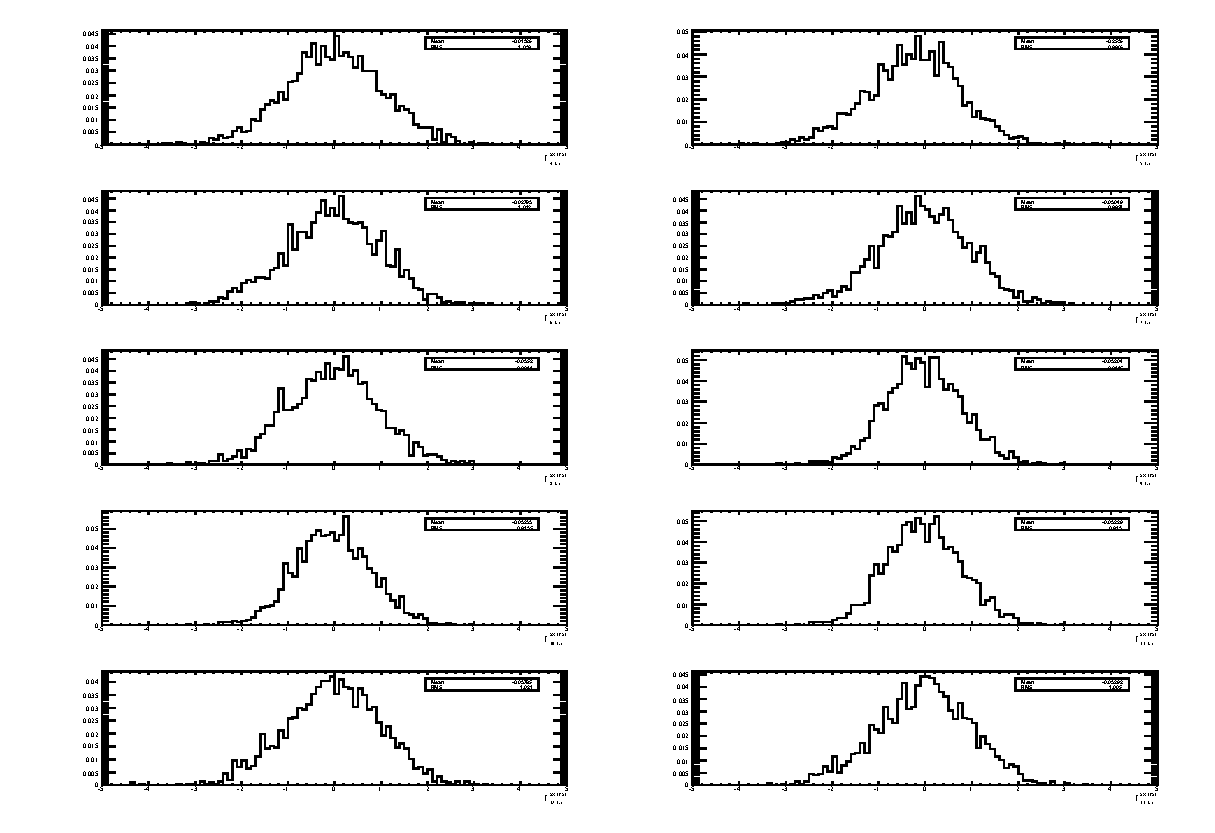
\includegraphics[width=1.0\textwidth]{images/validation/joint_pulls_point0_new_corr_hesse_pull_all_6.eps}
\caption{Distribution of pulls for the systematic parameters BANFF 4 - 13.
}
\label{fig:validation:pulls6}
\end{center}
\end{figure}

\begin{figure}[htbp]
\begin{center}
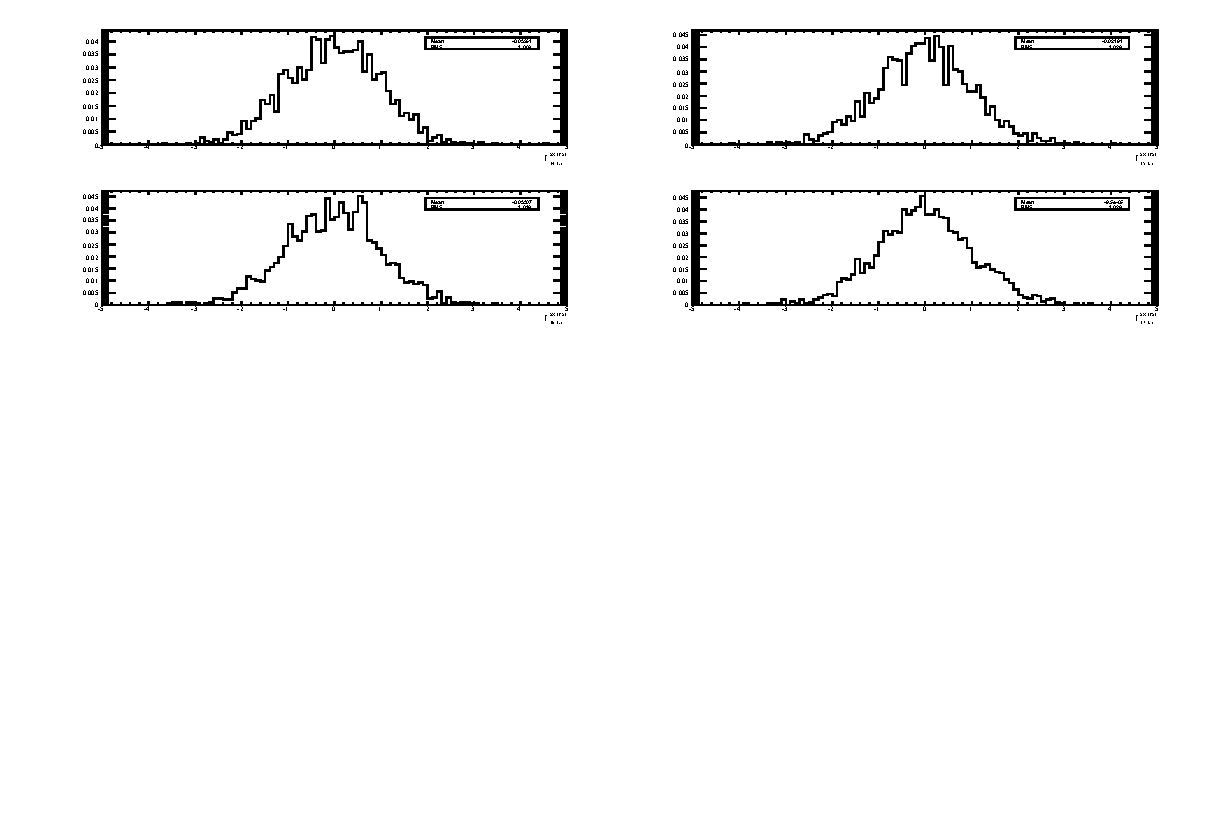
\includegraphics[width=1.0\textwidth]{images/validation/joint_pulls_point0_new_corr_hesse_pull_all_7.eps}
\caption{Distribution of pulls for the systematic parameters BANFF 14 - 17.
}
\label{fig:validation:pulls7}
\end{center}
\end{figure}


\begin{figure}[htbp]
\begin{center}
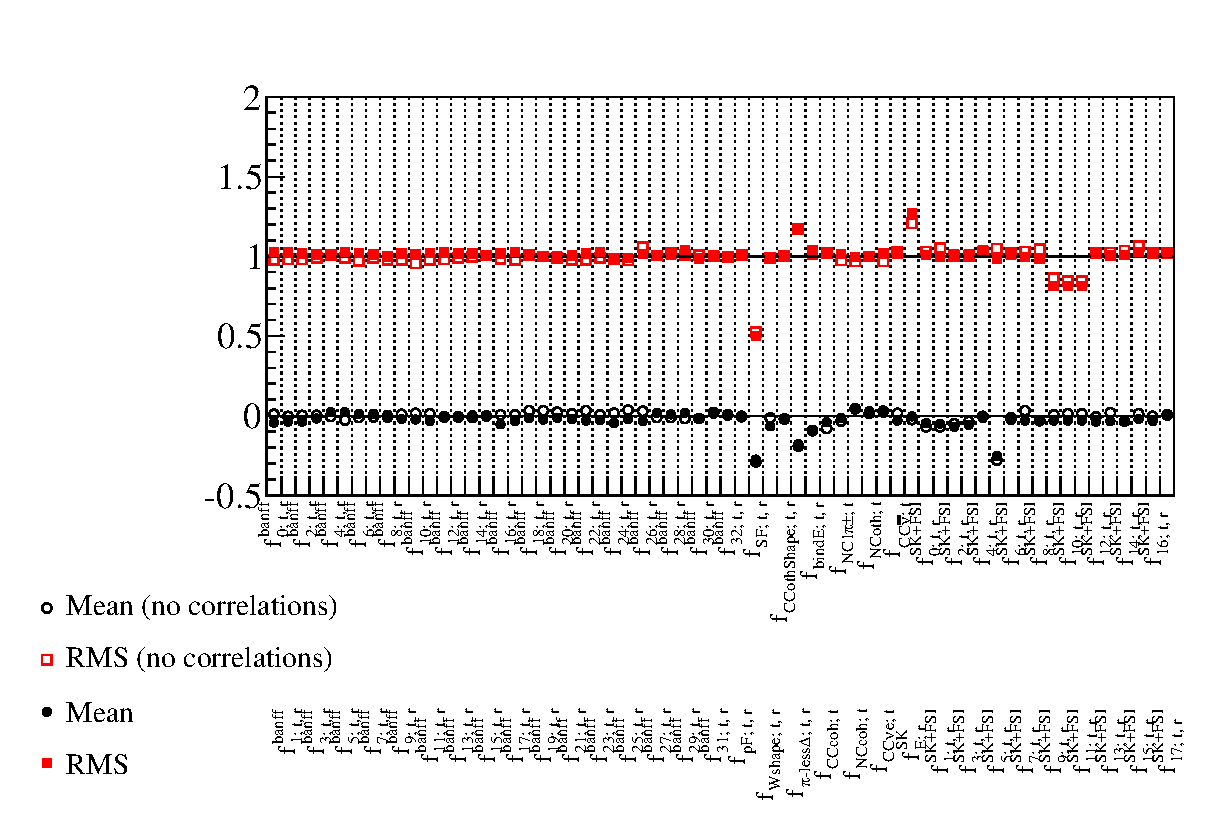
\includegraphics[width=1.0\textwidth, angle=270]{images/validation/Summary_pulls_systematics_final.eps}
\caption{Summary of mean and RMS for the distribution of pulls of the 64 systematic parameters with and without correlations.
}
\label{fig:validation:summary}
\end{center}
\end{figure}